\documentclass[1p]{elsarticle_modified}
%\bibliographystyle{elsarticle-num}

%\usepackage[colorlinks]{hyperref}
%\usepackage{abbrmath_seonhwa} %\Abb, \Ascr, \Acal ,\Abf, \Afrak
\usepackage{amsfonts}
\usepackage{amssymb}
\usepackage{amsmath}
\usepackage{amsthm}
\usepackage{scalefnt}
\usepackage{amsbsy}
\usepackage{kotex}
\usepackage{caption}
\usepackage{subfig}
\usepackage{color}
\usepackage{graphicx}
\usepackage{xcolor} %% white, black, red, green, blue, cyan, magenta, yellow
\usepackage{float}
\usepackage{setspace}
\usepackage{hyperref}

\usepackage{tikz}
\usetikzlibrary{arrows}

\usepackage{multirow}
\usepackage{array} % fixed length table
\usepackage{hhline}

%%%%%%%%%%%%%%%%%%%%%
\makeatletter
\renewcommand*\env@matrix[1][\arraystretch]{%
	\edef\arraystretch{#1}%
	\hskip -\arraycolsep
	\let\@ifnextchar\new@ifnextchar
	\array{*\c@MaxMatrixCols c}}
\makeatother %https://tex.stackexchange.com/questions/14071/how-can-i-increase-the-line-spacing-in-a-matrix
%%%%%%%%%%%%%%%

\usepackage[normalem]{ulem}

\newcommand{\msout}[1]{\ifmmode\text{\sout{\ensuremath{#1}}}\else\sout{#1}\fi}
%SOURCE: \msout is \stkout macro in https://tex.stackexchange.com/questions/20609/strikeout-in-math-mode

\newcommand{\cancel}[1]{
	\ifmmode
	{\color{red}\msout{#1}}
	\else
	{\color{red}\sout{#1}}
	\fi
}

\newcommand{\add}[1]{
	{\color{blue}\uwave{#1}}
}

\newcommand{\replace}[2]{
	\ifmmode
	{\color{red}\msout{#1}}{\color{blue}\uwave{#2}}
	\else
	{\color{red}\sout{#1}}{\color{blue}\uwave{#2}}
	\fi
}

\newcommand{\Sol}{\mathcal{S}} %segment
\newcommand{\D}{D} %diagram
\newcommand{\A}{\mathcal{A}} %arc


%%%%%%%%%%%%%%%%%%%%%%%%%%%%%5 test

\def\sl{\operatorname{\textup{SL}}(2,\Cbb)}
\def\psl{\operatorname{\textup{PSL}}(2,\Cbb)}
\def\quan{\mkern 1mu \triangleright \mkern 1mu}

\theoremstyle{definition}
\newtheorem{thm}{Theorem}[section]
\newtheorem{prop}[thm]{Proposition}
\newtheorem{lem}[thm]{Lemma}
\newtheorem{ques}[thm]{Question}
\newtheorem{cor}[thm]{Corollary}
\newtheorem{defn}[thm]{Definition}
\newtheorem{exam}[thm]{Example}
\newtheorem{rmk}[thm]{Remark}
\newtheorem{alg}[thm]{Algorithm}

\newcommand{\I}{\sqrt{-1}}
\begin{document}

%\begin{frontmatter}
%
%\title{Boundary parabolic representations of knots up to 8 crossings}
%
%%% Group authors per affiliation:
%\author{Yunhi Cho} 
%\address{Department of Mathematics, University of Seoul, Seoul, Korea}
%\ead{yhcho@uos.ac.kr}
%
%
%\author{Seonhwa Kim} %\fnref{s_kim}}
%\address{Center for Geometry and Physics, Institute for Basic Science, Pohang, 37673, Korea}
%\ead{ryeona17@ibs.re.kr}
%
%\author{Hyuk Kim}
%\address{Department of Mathematical Sciences, Seoul National University, Seoul 08826, Korea}
%\ead{hyukkim@snu.ac.kr}
%
%\author{Seokbeom Yoon}
%\address{Department of Mathematical Sciences, Seoul National University, Seoul, 08826,  Korea}
%\ead{sbyoon15@snu.ac.kr}
%
%\begin{abstract}
%We find all boundary parabolic representation of knots up to 8 crossings.
%
%\end{abstract}
%\begin{keyword}
%    \MSC[2010] 57M25 
%\end{keyword}
%
%\end{frontmatter}

%\linenumbers
%\tableofcontents
%
\newcommand\colored[1]{\textcolor{white}{\rule[-0.35ex]{0.8em}{1.4ex}}\kern-0.8em\color{red} #1}%
%\newcommand\colored[1]{\textcolor{white}{ #1}\kern-2.17ex	\textcolor{white}{ #1}\kern-1.81ex	\textcolor{white}{ #1}\kern-2.15ex\color{red}#1	}

{\Large $\underline{12n_{0877}~(K12n_{0877})}$}

\setlength{\tabcolsep}{10pt}
\renewcommand{\arraystretch}{1.6}
\vspace{1cm}\begin{tabular}{m{100pt}>{\centering\arraybackslash}m{274pt}}
\multirow{5}{120pt}{
	\centering
	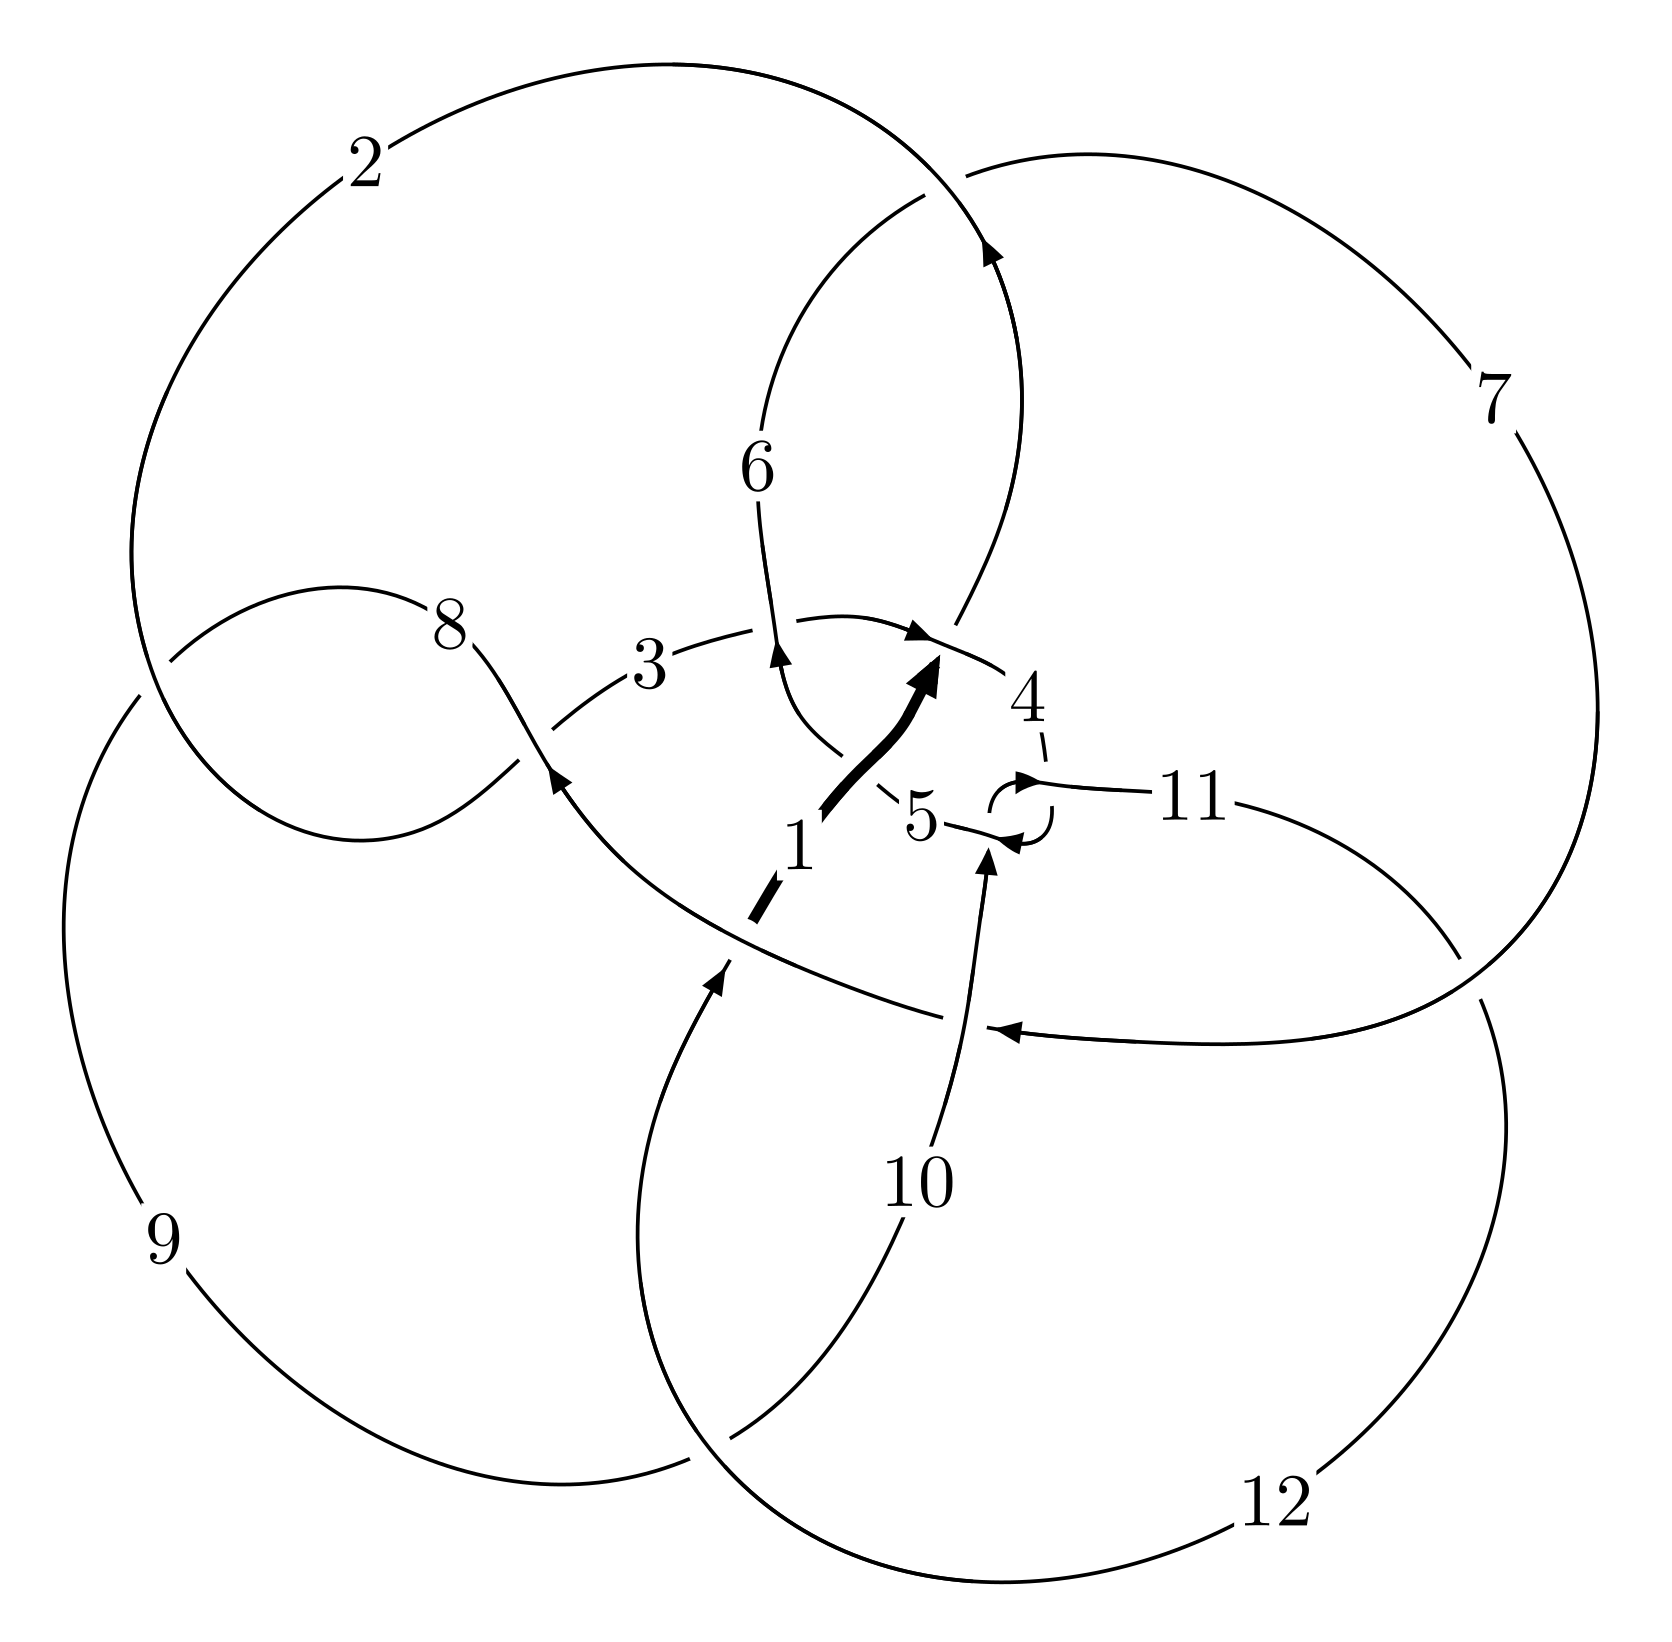
\includegraphics[width=112pt]{../../../GIT/diagram.site/Diagrams/png/2966_12n_0877.png}\\
\ \ \ A knot diagram\footnotemark}&
\allowdisplaybreaks
\textbf{Linearized knot diagam} \\
\cline{2-2}
 &
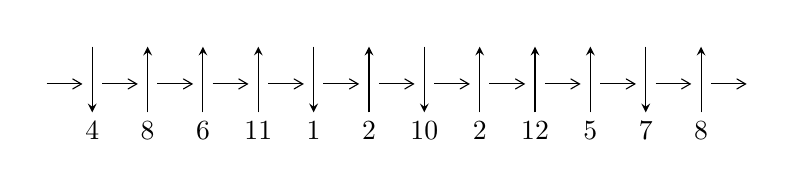
\begin{tikzpicture}[x=20pt, y=17pt]
	% nodes
	\node (C0) at (0, 0) {};
	\node (C1) at (1, 0) {};
	\node (C1U) at (1, +1) {};
	\node (C1D) at (1, -1) {4};

	\node (C2) at (2, 0) {};
	\node (C2U) at (2, +1) {};
	\node (C2D) at (2, -1) {8};

	\node (C3) at (3, 0) {};
	\node (C3U) at (3, +1) {};
	\node (C3D) at (3, -1) {6};

	\node (C4) at (4, 0) {};
	\node (C4U) at (4, +1) {};
	\node (C4D) at (4, -1) {11};

	\node (C5) at (5, 0) {};
	\node (C5U) at (5, +1) {};
	\node (C5D) at (5, -1) {1};

	\node (C6) at (6, 0) {};
	\node (C6U) at (6, +1) {};
	\node (C6D) at (6, -1) {2};

	\node (C7) at (7, 0) {};
	\node (C7U) at (7, +1) {};
	\node (C7D) at (7, -1) {10};

	\node (C8) at (8, 0) {};
	\node (C8U) at (8, +1) {};
	\node (C8D) at (8, -1) {2};

	\node (C9) at (9, 0) {};
	\node (C9U) at (9, +1) {};
	\node (C9D) at (9, -1) {12};

	\node (C10) at (10, 0) {};
	\node (C10U) at (10, +1) {};
	\node (C10D) at (10, -1) {5};

	\node (C11) at (11, 0) {};
	\node (C11U) at (11, +1) {};
	\node (C11D) at (11, -1) {7};

	\node (C12) at (12, 0) {};
	\node (C12U) at (12, +1) {};
	\node (C12D) at (12, -1) {8};
	\node (C13) at (13, 0) {};

	% arrows
	\draw[->,>={angle 60}]
	(C0) edge (C1) (C1) edge (C2) (C2) edge (C3) (C3) edge (C4) (C4) edge (C5) (C5) edge (C6) (C6) edge (C7) (C7) edge (C8) (C8) edge (C9) (C9) edge (C10) (C10) edge (C11) (C11) edge (C12) (C12) edge (C13) ;	\draw[->,>=stealth]
	(C1U) edge (C1D) (C2D) edge (C2U) (C3D) edge (C3U) (C4D) edge (C4U) (C5U) edge (C5D) (C6D) edge (C6U) (C7U) edge (C7D) (C8D) edge (C8U) (C9D) edge (C9U) (C10D) edge (C10U) (C11U) edge (C11D) (C12D) edge (C12U) ;
	\end{tikzpicture} \\
\hhline{~~} \\& 
\textbf{Solving Sequence} \\ \cline{2-2} 
 &
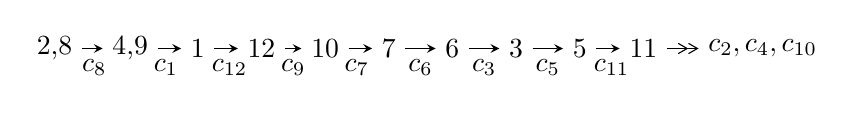
\begin{tikzpicture}[x=23pt, y=7pt]
	% node
	\node (A0) at (-1/8, 0) {2,8};
	\node (A1) at (17/16, 0) {4,9};
	\node (A2) at (17/8, 0) {1};
	\node (A3) at (25/8, 0) {12};
	\node (A4) at (33/8, 0) {10};
	\node (A5) at (41/8, 0) {7};
	\node (A6) at (49/8, 0) {6};
	\node (A7) at (57/8, 0) {3};
	\node (A8) at (65/8, 0) {5};
	\node (A9) at (73/8, 0) {11};
	\node (C1) at (1/2, -1) {$c_{8}$};
	\node (C2) at (13/8, -1) {$c_{1}$};
	\node (C3) at (21/8, -1) {$c_{12}$};
	\node (C4) at (29/8, -1) {$c_{9}$};
	\node (C5) at (37/8, -1) {$c_{7}$};
	\node (C6) at (45/8, -1) {$c_{6}$};
	\node (C7) at (53/8, -1) {$c_{3}$};
	\node (C8) at (61/8, -1) {$c_{5}$};
	\node (C9) at (69/8, -1) {$c_{11}$};
	\node (A10) at (11, 0) {$c_{2},c_{4},c_{10}$};

	% edge
	\draw[->,>=stealth]	
	(A0) edge (A1) (A1) edge (A2) (A2) edge (A3) (A3) edge (A4) (A4) edge (A5) (A5) edge (A6) (A6) edge (A7) (A7) edge (A8) (A8) edge (A9) ;
	\draw[->>,>={angle 60}]	
	(A9) edge (A10);
\end{tikzpicture} \\ 

\end{tabular} \\

\footnotetext{
The image of knot diagram is generated by the software ``\textbf{Draw programme}" developed by Andrew Bartholomew(\url{http://www.layer8.co.uk/maths/draw/index.htm\#Running-draw}), where we modified some parts for our purpose(\url{https://github.com/CATsTAILs/LinksPainter}).
}\phantom \\ \newline 
\centering \textbf{Ideals for irreducible components\footnotemark of $X_{\text{par}}$} 
 
\begin{align*}
I^u_{1}&=\langle 
-9.35659\times10^{83} u^{36}-2.27819\times10^{84} u^{35}+\cdots+9.11104\times10^{86} b+1.23806\times10^{87},\\
\phantom{I^u_{1}}&\phantom{= \langle  }-2.69779\times10^{87} u^{36}-1.19660\times10^{88} u^{35}+\cdots+1.76754\times10^{89} a-1.89107\times10^{90},\\
\phantom{I^u_{1}}&\phantom{= \langle  }u^{37}+5 u^{36}+\cdots+2744 u+388\rangle \\
I^u_{2}&=\langle 
3.32625\times10^{77} a u^{42}-3.27571\times10^{78} u^{42}+\cdots+1.71826\times10^{79} a-1.65861\times10^{80},\\
\phantom{I^u_{2}}&\phantom{= \langle  }5.05212\times10^{81} a u^{42}-1.09660\times10^{82} u^{42}+\cdots+1.99839\times10^{83} a-3.99060\times10^{83},\\
\phantom{I^u_{2}}&\phantom{= \langle  }u^{43}-3 u^{42}+\cdots+110 u-17\rangle \\
I^u_{3}&=\langle 
2.20191\times10^{25} u^{39}+2.35786\times10^{25} u^{38}+\cdots+1.03004\times10^{24} b-1.37061\times10^{27},\\
\phantom{I^u_{3}}&\phantom{= \langle  }-7.73943\times10^{26} u^{39}-1.52201\times10^{26} u^{38}+\cdots+1.95708\times10^{25} a+9.28110\times10^{27},\\
\phantom{I^u_{3}}&\phantom{= \langle  }u^{40}-6 u^{38}+\cdots-255 u^2-19\rangle \\
I^u_{4}&=\langle 
b,\;a^2- a+1,\;u+1\rangle \\
I^u_{5}&=\langle 
b-2 a,\;a^2- a+1,\;u-1\rangle \\
\\
I^v_{1}&=\langle 
a,\;b^2+b+1,\;v+1\rangle \\
\end{align*}
\raggedright * 6 irreducible components of $\dim_{\mathbb{C}}=0$, with total 169 representations.\\
\footnotetext{All coefficients of polynomials are rational numbers. But the coefficients are sometimes approximated in decimal forms when there is not enough margin.}
\newpage
\renewcommand{\arraystretch}{1}
\centering \section*{I. $I^u_{1}= \langle -9.36\times10^{83} u^{36}-2.28\times10^{84} u^{35}+\cdots+9.11\times10^{86} b+1.24\times10^{87},\;-2.70\times10^{87} u^{36}-1.20\times10^{88} u^{35}+\cdots+1.77\times10^{89} a-1.89\times10^{90},\;u^{37}+5 u^{36}+\cdots+2744 u+388 \rangle$}
\flushleft \textbf{(i) Arc colorings}\\
\begin{tabular}{m{7pt} m{180pt} m{7pt} m{180pt} }
\flushright $a_{2}=$&$\begin{pmatrix}0\\u\end{pmatrix}$ \\
\flushright $a_{8}=$&$\begin{pmatrix}1\\0\end{pmatrix}$ \\
\flushright $a_{4}=$&$\begin{pmatrix}0.0152630 u^{36}+0.0676983 u^{35}+\cdots+58.5223 u+10.6989\\0.00102695 u^{36}+0.00250048 u^{35}+\cdots-1.09050 u-1.35885\end{pmatrix}$ \\
\flushright $a_{9}=$&$\begin{pmatrix}1\\- u^2\end{pmatrix}$ \\
\flushright $a_{1}=$&$\begin{pmatrix}0.0180233 u^{36}+0.0813561 u^{35}+\cdots+78.6888 u+17.0783\\0.00546745 u^{36}+0.0219598 u^{35}+\cdots+15.1454 u+2.22914\end{pmatrix}$ \\
\flushright $a_{12}=$&$\begin{pmatrix}0.0125559 u^{36}+0.0593963 u^{35}+\cdots+63.5435 u+14.8491\\0.00546745 u^{36}+0.0219598 u^{35}+\cdots+15.1454 u+2.22914\end{pmatrix}$ \\
\flushright $a_{10}=$&$\begin{pmatrix}0.00350220 u^{36}+0.0185379 u^{35}+\cdots+25.9914 u+8.51953\\0.00861657 u^{36}+0.0375921 u^{35}+\cdots+31.1827 u+5.92203\end{pmatrix}$ \\
\flushright $a_{7}=$&$\begin{pmatrix}-0.00574521 u^{36}-0.0232586 u^{35}+\cdots-14.5732 u-0.619490\\0.00876059 u^{36}+0.0373042 u^{35}+\cdots+32.3778 u+6.99306\end{pmatrix}$ \\
\flushright $a_{6}=$&$\begin{pmatrix}-0.00574521 u^{36}-0.0232586 u^{35}+\cdots-14.5732 u-0.619490\\0.00338316 u^{36}+0.0164838 u^{35}+\cdots+19.6043 u+4.87169\end{pmatrix}$ \\
\flushright $a_{3}=$&$\begin{pmatrix}u\\u\end{pmatrix}$ \\
\flushright $a_{5}=$&$\begin{pmatrix}0.0216125 u^{36}+0.0975640 u^{35}+\cdots+96.4003 u+24.3397\\0.0235451 u^{36}+0.0984750 u^{35}+\cdots+81.0110 u+16.7723\end{pmatrix}$ \\
\flushright $a_{11}=$&$\begin{pmatrix}0.0432275 u^{36}+0.192592 u^{35}+\cdots+178.923 u+37.6052\\-0.0104986 u^{36}-0.0434372 u^{35}+\cdots-34.9650 u-8.38565\end{pmatrix}$\\&\end{tabular}
\flushleft \textbf{(ii) Obstruction class $= -1$}\\~\\
\flushleft \textbf{(iii) Cusp Shapes $= -0.0638114 u^{36}-0.256490 u^{35}+\cdots-174.364 u-30.2157$}\\~\\
\newpage\renewcommand{\arraystretch}{1}
\flushleft \textbf{(iv) u-Polynomials at the component}\newline \\
\begin{tabular}{m{50pt}|m{274pt}}
Crossings & \hspace{64pt}u-Polynomials at each crossing \\
\hline $$\begin{aligned}c_{1},c_{7}\end{aligned}$$&$\begin{aligned}
&u^{37}- u^{36}+\cdots+8 u-1
\end{aligned}$\\
\hline $$\begin{aligned}c_{2},c_{8}\end{aligned}$$&$\begin{aligned}
&u^{37}+5 u^{36}+\cdots+2744 u+388
\end{aligned}$\\
\hline $$\begin{aligned}c_{3},c_{9}\end{aligned}$$&$\begin{aligned}
&u^{37}+u^{36}+\cdots+2 u+1
\end{aligned}$\\
\hline $$\begin{aligned}c_{4},c_{10}\end{aligned}$$&$\begin{aligned}
&u^{37}+5 u^{36}+\cdots+184 u+52
\end{aligned}$\\
\hline $$\begin{aligned}c_{5},c_{11}\end{aligned}$$&$\begin{aligned}
&u^{37}+u^{36}+\cdots-4 u+4
\end{aligned}$\\
\hline $$\begin{aligned}c_{6},c_{12}\end{aligned}$$&$\begin{aligned}
&u^{37}- u^{36}+\cdots-104 u-47
\end{aligned}$\\
\hline
\end{tabular}\\~\\
\newpage\renewcommand{\arraystretch}{1}
\flushleft \textbf{(v) Riley Polynomials at the component}\newline \\
\begin{tabular}{m{50pt}|m{274pt}}
Crossings & \hspace{64pt}Riley Polynomials at each crossing \\
\hline $$\begin{aligned}c_{1},c_{7}\end{aligned}$$&$\begin{aligned}
&y^{37}-11 y^{36}+\cdots+32 y-1
\end{aligned}$\\
\hline $$\begin{aligned}c_{2},c_{8}\end{aligned}$$&$\begin{aligned}
&y^{37}-23 y^{36}+\cdots+3132720 y-150544
\end{aligned}$\\
\hline $$\begin{aligned}c_{3},c_{9}\end{aligned}$$&$\begin{aligned}
&y^{37}-37 y^{36}+\cdots+30 y-1
\end{aligned}$\\
\hline $$\begin{aligned}c_{4},c_{10}\end{aligned}$$&$\begin{aligned}
&y^{37}+13 y^{36}+\cdots-5872 y-2704
\end{aligned}$\\
\hline $$\begin{aligned}c_{5},c_{11}\end{aligned}$$&$\begin{aligned}
&y^{37}-5 y^{36}+\cdots-976 y-16
\end{aligned}$\\
\hline $$\begin{aligned}c_{6},c_{12}\end{aligned}$$&$\begin{aligned}
&y^{37}-31 y^{36}+\cdots+16456 y-2209
\end{aligned}$\\
\hline
\end{tabular}\\~\\
\newpage\flushleft \textbf{(vi) Complex Volumes and Cusp Shapes}
$$\begin{array}{c|c|c}  
\text{Solutions to }I^u_{1}& \I (\text{vol} + \sqrt{-1}CS) & \text{Cusp shape}\\
 \hline 
\begin{aligned}
u &= -1.023680 + 0.207468 I \\
a &= -0.224911 + 0.827302 I \\
b &= \phantom{-}0.956147 + 0.338744 I\end{aligned}
 & \phantom{-}5.14523 - 0.88050 I & \phantom{-}13.89731 - 1.40909 I \\ \hline\begin{aligned}
u &= -1.023680 - 0.207468 I \\
a &= -0.224911 - 0.827302 I \\
b &= \phantom{-}0.956147 - 0.338744 I\end{aligned}
 & \phantom{-}5.14523 + 0.88050 I & \phantom{-}13.89731 + 1.40909 I \\ \hline\begin{aligned}
u &= -0.513603 + 0.927764 I \\
a &= -0.362915 + 1.130270 I \\
b &= -0.266581 + 1.169590 I\end{aligned}
 & -2.71819 - 6.93203 I & \phantom{-}1.49325 + 6.38376 I \\ \hline\begin{aligned}
u &= -0.513603 - 0.927764 I \\
a &= -0.362915 - 1.130270 I \\
b &= -0.266581 - 1.169590 I\end{aligned}
 & -2.71819 + 6.93203 I & \phantom{-}1.49325 - 6.38376 I \\ \hline\begin{aligned}
u &= -0.203243 + 0.874057 I \\
a &= \phantom{-}0.21000 + 1.77056 I \\
b &= -0.05883 + 1.53025 I\end{aligned}
 & -5.67964 + 1.01449 I & \phantom{-}4.29448 - 6.92334 I \\ \hline\begin{aligned}
u &= -0.203243 - 0.874057 I \\
a &= \phantom{-}0.21000 - 1.77056 I \\
b &= -0.05883 - 1.53025 I\end{aligned}
 & -5.67964 - 1.01449 I & \phantom{-}4.29448 + 6.92334 I \\ \hline\begin{aligned}
u &= \phantom{-}0.393345 + 0.759798 I \\
a &= \phantom{-}0.341465 + 0.953652 I \\
b &= \phantom{-}0.130643 + 0.919943 I\end{aligned}
 & -0.18355 + 2.03501 I & \phantom{-}3.27155 - 3.11294 I \\ \hline\begin{aligned}
u &= \phantom{-}0.393345 - 0.759798 I \\
a &= \phantom{-}0.341465 - 0.953652 I \\
b &= \phantom{-}0.130643 - 0.919943 I\end{aligned}
 & -0.18355 - 2.03501 I & \phantom{-}3.27155 + 3.11294 I \\ \hline\begin{aligned}
u &= -0.259763 + 1.213030 I \\
a &= \phantom{-}0.172358 + 0.907964 I \\
b &= \phantom{-}0.13042 + 1.58902 I\end{aligned}
 & -5.01261 + 1.59452 I & -0.74857 - 4.14264 I \\ \hline\begin{aligned}
u &= -0.259763 - 1.213030 I \\
a &= \phantom{-}0.172358 - 0.907964 I \\
b &= \phantom{-}0.13042 - 1.58902 I\end{aligned}
 & -5.01261 - 1.59452 I & -0.74857 + 4.14264 I\\
 \hline 
 \end{array}$$\newpage$$\begin{array}{c|c|c}  
\text{Solutions to }I^u_{1}& \I (\text{vol} + \sqrt{-1}CS) & \text{Cusp shape}\\
 \hline 
\begin{aligned}
u &= \phantom{-}1.255890 + 0.068162 I \\
a &= -0.132967 + 0.395325 I \\
b &= -1.177290 + 0.087112 I\end{aligned}
 & \phantom{-}3.63356 + 3.81297 I & \phantom{-}10.07806 - 5.49647 I \\ \hline\begin{aligned}
u &= \phantom{-}1.255890 - 0.068162 I \\
a &= -0.132967 - 0.395325 I \\
b &= -1.177290 - 0.087112 I\end{aligned}
 & \phantom{-}3.63356 - 3.81297 I & \phantom{-}10.07806 + 5.49647 I \\ \hline\begin{aligned}
u &= -0.452009 + 0.440661 I \\
a &= \phantom{-}1.136500 + 0.492247 I \\
b &= -0.989885 - 0.684757 I\end{aligned}
 & -1.67227 + 2.60991 I & -2.01632 - 5.81175 I \\ \hline\begin{aligned}
u &= -0.452009 - 0.440661 I \\
a &= \phantom{-}1.136500 - 0.492247 I \\
b &= -0.989885 + 0.684757 I\end{aligned}
 & -1.67227 - 2.60991 I & -2.01632 + 5.81175 I \\ \hline\begin{aligned}
u &= -1.381620 + 0.001380 I \\
a &= -0.716115 + 0.134351 I \\
b &= -0.596037 + 0.248959 I\end{aligned}
 & \phantom{-}0.77318 + 3.37059 I & -2.04958 - 4.00982 I \\ \hline\begin{aligned}
u &= -1.381620 - 0.001380 I \\
a &= -0.716115 - 0.134351 I \\
b &= -0.596037 - 0.248959 I\end{aligned}
 & \phantom{-}0.77318 - 3.37059 I & -2.04958 + 4.00982 I \\ \hline\begin{aligned}
u &= \phantom{-}1.45601\phantom{ +0.000000I} \\
a &= \phantom{-}0.621894\phantom{ +0.000000I} \\
b &= \phantom{-}0.272503\phantom{ +0.000000I}\end{aligned}
 & \phantom{-}3.33967\phantom{ +0.000000I} & \phantom{-}2.87470\phantom{ +0.000000I} \\ \hline\begin{aligned}
u &= \phantom{-}0.473903 + 0.174617 I \\
a &= \phantom{-}0.614985 + 0.716675 I \\
b &= \phantom{-}0.514605 + 0.316308 I\end{aligned}
 & \phantom{-}1.022900 + 0.779663 I & \phantom{-}7.50935 - 3.53502 I \\ \hline\begin{aligned}
u &= \phantom{-}0.473903 - 0.174617 I \\
a &= \phantom{-}0.614985 - 0.716675 I \\
b &= \phantom{-}0.514605 - 0.316308 I\end{aligned}
 & \phantom{-}1.022900 - 0.779663 I & \phantom{-}7.50935 + 3.53502 I \\ \hline\begin{aligned}
u &= -0.04479 + 1.52449 I \\
a &= -0.568234 + 0.602533 I \\
b &= \phantom{-}0.29065 + 1.60332 I\end{aligned}
 & \phantom{-}2.46403 - 4.84771 I & \phantom{-}7.83065 + 5.43608 I\\
 \hline 
 \end{array}$$\newpage$$\begin{array}{c|c|c}  
\text{Solutions to }I^u_{1}& \I (\text{vol} + \sqrt{-1}CS) & \text{Cusp shape}\\
 \hline 
\begin{aligned}
u &= -0.04479 - 1.52449 I \\
a &= -0.568234 - 0.602533 I \\
b &= \phantom{-}0.29065 - 1.60332 I\end{aligned}
 & \phantom{-}2.46403 + 4.84771 I & \phantom{-}7.83065 - 5.43608 I \\ \hline\begin{aligned}
u &= -1.53849 + 0.44250 I \\
a &= -0.509830 - 0.453544 I \\
b &= \phantom{-}1.61671 - 1.81990 I\end{aligned}
 & -0.30645 - 7.70638 I & \phantom{-0.000000 -}0. + 7.90475 I \\ \hline\begin{aligned}
u &= -1.53849 - 0.44250 I \\
a &= -0.509830 + 0.453544 I \\
b &= \phantom{-}1.61671 + 1.81990 I\end{aligned}
 & -0.30645 + 7.70638 I & \phantom{-0.000000 } 0. - 7.90475 I \\ \hline\begin{aligned}
u &= -0.353652 + 0.059931 I \\
a &= -1.80596 + 0.93479 I \\
b &= -0.562272 - 0.178009 I\end{aligned}
 & -0.91481 + 3.77913 I & \phantom{-}5.64104 - 2.45174 I \\ \hline\begin{aligned}
u &= -0.353652 - 0.059931 I \\
a &= -1.80596 - 0.93479 I \\
b &= -0.562272 + 0.178009 I\end{aligned}
 & -0.91481 - 3.77913 I & \phantom{-}5.64104 + 2.45174 I \\ \hline\begin{aligned}
u &= -1.67250\phantom{ +0.000000I} \\
a &= -0.101046\phantom{ +0.000000I} \\
b &= \phantom{-}2.66187\phantom{ +0.000000I}\end{aligned}
 & \phantom{-}8.44157\phantom{ +0.000000I} & \phantom{-}14.5320\phantom{ +0.000000I} \\ \hline\begin{aligned}
u &= -1.45646 + 0.84376 I \\
a &= -0.737564 + 0.407660 I \\
b &= \phantom{-}0.303225 + 0.408038 I\end{aligned}
 & \phantom{-}6.74334 - 2.70316 I & \phantom{-0.000000 } 0 \\ \hline\begin{aligned}
u &= -1.45646 - 0.84376 I \\
a &= -0.737564 - 0.407660 I \\
b &= \phantom{-}0.303225 - 0.408038 I\end{aligned}
 & \phantom{-}6.74334 + 2.70316 I & \phantom{-0.000000 } 0 \\ \hline\begin{aligned}
u &= \phantom{-}1.74832\phantom{ +0.000000I} \\
a &= \phantom{-}0.405395\phantom{ +0.000000I} \\
b &= -3.70278\phantom{ +0.000000I}\end{aligned}
 & \phantom{-}7.10544\phantom{ +0.000000I} & \phantom{-0.000000 } 0 \\ \hline\begin{aligned}
u &= -0.00849 + 1.76143 I \\
a &= \phantom{-}0.643665 + 0.717640 I \\
b &= -0.11867 + 1.49405 I\end{aligned}
 & -0.02411 + 10.88880 I & \phantom{-0.000000 } 0\\
 \hline 
 \end{array}$$\newpage$$\begin{array}{c|c|c}  
\text{Solutions to }I^u_{1}& \I (\text{vol} + \sqrt{-1}CS) & \text{Cusp shape}\\
 \hline 
\begin{aligned}
u &= -0.00849 - 1.76143 I \\
a &= \phantom{-}0.643665 - 0.717640 I \\
b &= -0.11867 - 1.49405 I\end{aligned}
 & -0.02411 - 10.88880 I & \phantom{-0.000000 } 0 \\ \hline\begin{aligned}
u &= \phantom{-}1.66398 + 0.63157 I \\
a &= \phantom{-}0.300742 - 0.721731 I \\
b &= -0.84961 - 2.41654 I\end{aligned}
 & \phantom{-}8.0218 + 12.6732 I & \phantom{-0.000000 } 0 \\ \hline\begin{aligned}
u &= \phantom{-}1.66398 - 0.63157 I \\
a &= \phantom{-}0.300742 + 0.721731 I \\
b &= -0.84961 + 2.41654 I\end{aligned}
 & \phantom{-}8.0218 - 12.6732 I & \phantom{-0.000000 } 0 \\ \hline\begin{aligned}
u &= -1.66761 + 0.70883 I \\
a &= -0.330845 - 0.831651 I \\
b &= \phantom{-}0.67399 - 2.28474 I\end{aligned}
 & \phantom{-}5.3307 - 19.4688 I & \phantom{-0.000000 } 0 \\ \hline\begin{aligned}
u &= -1.66761 - 0.70883 I \\
a &= -0.330845 + 0.831651 I \\
b &= \phantom{-}0.67399 + 2.28474 I\end{aligned}
 & \phantom{-}5.3307 + 19.4688 I & \phantom{-0.000000 } 0 \\ \hline\begin{aligned}
u &= \phantom{-}1.85036 + 0.61716 I \\
a &= \phantom{-}0.769394 + 0.240989 I \\
b &= -0.113001 + 0.215300 I\end{aligned}
 & \phantom{-}6.00980 - 1.88404 I & \phantom{-0.000000 } 0 \\ \hline\begin{aligned}
u &= \phantom{-}1.85036 - 0.61716 I \\
a &= \phantom{-}0.769394 - 0.240989 I \\
b &= -0.113001 - 0.215300 I\end{aligned}
 & \phantom{-}6.00980 + 1.88404 I & \phantom{-0.000000 } 0\\
 \hline 
 \end{array}$$\newpage\newpage\renewcommand{\arraystretch}{1}
\centering \section*{II. $I^u_{2}= \langle 3.33\times10^{77} a u^{42}-3.28\times10^{78} u^{42}+\cdots+1.72\times10^{79} a-1.66\times10^{80},\;5.05\times10^{81} a u^{42}-1.10\times10^{82} u^{42}+\cdots+2.00\times10^{83} a-3.99\times10^{83},\;u^{43}-3 u^{42}+\cdots+110 u-17 \rangle$}
\flushleft \textbf{(i) Arc colorings}\\
\begin{tabular}{m{7pt} m{180pt} m{7pt} m{180pt} }
\flushright $a_{2}=$&$\begin{pmatrix}0\\u\end{pmatrix}$ \\
\flushright $a_{8}=$&$\begin{pmatrix}1\\0\end{pmatrix}$ \\
\flushright $a_{4}=$&$\begin{pmatrix}a\\-0.00287322 a u^{42}+0.0282956 u^{42}+\cdots-0.148423 a+1.43271\end{pmatrix}$ \\
\flushright $a_{9}=$&$\begin{pmatrix}1\\- u^2\end{pmatrix}$ \\
\flushright $a_{1}=$&$\begin{pmatrix}-0.0460162 a u^{42}+0.106090 u^{42}+\cdots-2.56707 a+5.57201\\0.00293218 a u^{42}-0.0252712 u^{42}+\cdots+0.473351 a-0.516706\end{pmatrix}$ \\
\flushright $a_{12}=$&$\begin{pmatrix}-0.0489483 a u^{42}+0.131361 u^{42}+\cdots-3.04042 a+6.08871\\0.00293218 a u^{42}-0.0252712 u^{42}+\cdots+0.473351 a-0.516706\end{pmatrix}$ \\
\flushright $a_{10}=$&$\begin{pmatrix}0.00873077 a u^{42}+0.106037 u^{42}+\cdots-1.17990 a+5.44946\\0.0460162 u^{42}-0.137175 u^{41}+\cdots-10.6374 u+2.56707\end{pmatrix}$ \\
\flushright $a_{7}=$&$\begin{pmatrix}-0.0278442 a u^{42}-0.0717915 u^{42}+\cdots-1.80262 a-7.63595\\-0.000873541 a u^{42}-0.0982682 u^{42}+\cdots-0.782275 a-4.47485\end{pmatrix}$ \\
\flushright $a_{6}=$&$\begin{pmatrix}-0.0278442 a u^{42}-0.0717915 u^{42}+\cdots-1.80262 a-7.63595\\-0.00293545 a u^{42}-0.0837892 u^{42}+\cdots-0.832122 a-3.94930\end{pmatrix}$ \\
\flushright $a_{3}=$&$\begin{pmatrix}u\\u\end{pmatrix}$ \\
\flushright $a_{5}=$&$\begin{pmatrix}0.00984394 a u^{42}-0.125943 u^{42}+\cdots+1.79971 a-5.22417\\0.00422200 a u^{42}-0.0543645 u^{42}+\cdots-0.723111 a-3.46387\end{pmatrix}$ \\
\flushright $a_{11}=$&$\begin{pmatrix}-0.0425359 a u^{42}-0.0109791 u^{42}+\cdots-3.72010 a+0.0400840\\-0.00613998 a u^{42}-0.0134470 u^{42}+\cdots-0.167347 a-0.720202\end{pmatrix}$\\&\end{tabular}
\flushleft \textbf{(ii) Obstruction class $= -1$}\\~\\
\flushleft \textbf{(iii) Cusp Shapes $= 0.260099 u^{42}-0.756964 u^{41}+\cdots-62.4522 u+23.1375$}\\~\\
\newpage\renewcommand{\arraystretch}{1}
\flushleft \textbf{(iv) u-Polynomials at the component}\newline \\
\begin{tabular}{m{50pt}|m{274pt}}
Crossings & \hspace{64pt}u-Polynomials at each crossing \\
\hline $$\begin{aligned}c_{1},c_{7}\end{aligned}$$&$\begin{aligned}
&u^{86}-7 u^{85}+\cdots-55 u+3
\end{aligned}$\\
\hline $$\begin{aligned}c_{2},c_{8}\end{aligned}$$&$\begin{aligned}
&(u^{43}-3 u^{42}+\cdots+110 u-17)^{2}
\end{aligned}$\\
\hline $$\begin{aligned}c_{3},c_{9}\end{aligned}$$&$\begin{aligned}
&u^{86}+4 u^{85}+\cdots+3742879 u+515187
\end{aligned}$\\
\hline $$\begin{aligned}c_{4},c_{10}\end{aligned}$$&$\begin{aligned}
&(u^{43}-2 u^{42}+\cdots+8 u-5)^{2}
\end{aligned}$\\
\hline $$\begin{aligned}c_{5},c_{11}\end{aligned}$$&$\begin{aligned}
&u^{86}+2 u^{85}+\cdots-1380 u+529
\end{aligned}$\\
\hline $$\begin{aligned}c_{6},c_{12}\end{aligned}$$&$\begin{aligned}
&u^{86}-2 u^{85}+\cdots+2676206273 u+339660187
\end{aligned}$\\
\hline
\end{tabular}\\~\\
\newpage\renewcommand{\arraystretch}{1}
\flushleft \textbf{(v) Riley Polynomials at the component}\newline \\
\begin{tabular}{m{50pt}|m{274pt}}
Crossings & \hspace{64pt}Riley Polynomials at each crossing \\
\hline $$\begin{aligned}c_{1},c_{7}\end{aligned}$$&$\begin{aligned}
&y^{86}-7 y^{85}+\cdots-31 y+9
\end{aligned}$\\
\hline $$\begin{aligned}c_{2},c_{8}\end{aligned}$$&$\begin{aligned}
&(y^{43}-39 y^{42}+\cdots+4960 y-289)^{2}
\end{aligned}$\\
\hline $$\begin{aligned}c_{3},c_{9}\end{aligned}$$&$\begin{aligned}
&y^{86}-28 y^{85}+\cdots-1722726646621 y+265417644969
\end{aligned}$\\
\hline $$\begin{aligned}c_{4},c_{10}\end{aligned}$$&$\begin{aligned}
&(y^{43}+20 y^{42}+\cdots-446 y-25)^{2}
\end{aligned}$\\
\hline $$\begin{aligned}c_{5},c_{11}\end{aligned}$$&$\begin{aligned}
&y^{86}+32 y^{85}+\cdots+34272852 y+279841
\end{aligned}$\\
\hline $$\begin{aligned}c_{6},c_{12}\end{aligned}$$&$\begin{aligned}
&y^{86}-10 y^{85}+\cdots-3384577457419862375 y+115369042632874969
\end{aligned}$\\
\hline
\end{tabular}\\~\\
\newpage\flushleft \textbf{(vi) Complex Volumes and Cusp Shapes}
$$\begin{array}{c|c|c}  
\text{Solutions to }I^u_{2}& \I (\text{vol} + \sqrt{-1}CS) & \text{Cusp shape}\\
 \hline 
\begin{aligned}
u &= -1.115680 + 0.088438 I \\
a &= -0.530621 - 0.816347 I \\
b &= -0.36669 - 1.40614 I\end{aligned}
 & \phantom{-}2.05988 - 4.53064 I & \phantom{-}6.07841 + 4.88354 I \\ \hline\begin{aligned}
u &= -1.115680 + 0.088438 I \\
a &= \phantom{-}0.016420 + 0.564275 I \\
b &= -0.685045 - 0.446535 I\end{aligned}
 & \phantom{-}2.05988 - 4.53064 I & \phantom{-}6.07841 + 4.88354 I \\ \hline\begin{aligned}
u &= -1.115680 - 0.088438 I \\
a &= -0.530621 + 0.816347 I \\
b &= -0.36669 + 1.40614 I\end{aligned}
 & \phantom{-}2.05988 + 4.53064 I & \phantom{-}6.07841 - 4.88354 I \\ \hline\begin{aligned}
u &= -1.115680 - 0.088438 I \\
a &= \phantom{-}0.016420 - 0.564275 I \\
b &= -0.685045 + 0.446535 I\end{aligned}
 & \phantom{-}2.05988 + 4.53064 I & \phantom{-}6.07841 - 4.88354 I \\ \hline\begin{aligned}
u &= \phantom{-}1.194820 + 0.508478 I \\
a &= \phantom{-}0.529082 + 0.865996 I \\
b &= -0.128273 + 0.357532 I\end{aligned}
 & \phantom{-}3.19067 + 2.37658 I & \phantom{-0.000000 } 0. - 11.61854 I \\ \hline\begin{aligned}
u &= \phantom{-}1.194820 + 0.508478 I \\
a &= \phantom{-}0.127113 - 0.366982 I \\
b &= -2.67295 - 2.83110 I\end{aligned}
 & \phantom{-}3.19067 + 2.37658 I & \phantom{-0.000000 } 0. - 11.61854 I \\ \hline\begin{aligned}
u &= \phantom{-}1.194820 - 0.508478 I \\
a &= \phantom{-}0.529082 - 0.865996 I \\
b &= -0.128273 - 0.357532 I\end{aligned}
 & \phantom{-}3.19067 - 2.37658 I & \phantom{-0.000000 -}0. + 11.61854 I \\ \hline\begin{aligned}
u &= \phantom{-}1.194820 - 0.508478 I \\
a &= \phantom{-}0.127113 + 0.366982 I \\
b &= -2.67295 + 2.83110 I\end{aligned}
 & \phantom{-}3.19067 - 2.37658 I & \phantom{-0.000000 -}0. + 11.61854 I \\ \hline\begin{aligned}
u &= \phantom{-}1.337540 + 0.195957 I \\
a &= \phantom{-}0.751109 - 0.509623 I \\
b &= \phantom{-}0.64184 - 1.29054 I\end{aligned}
 & \phantom{-}0.786358 + 1.135550 I & \phantom{-0.000000 } 0 \\ \hline\begin{aligned}
u &= \phantom{-}1.337540 + 0.195957 I \\
a &= -0.162295 - 0.099306 I \\
b &= \phantom{-}0.298914 - 0.668145 I\end{aligned}
 & \phantom{-}0.786358 + 1.135550 I & \phantom{-0.000000 } 0\\
 \hline 
 \end{array}$$\newpage$$\begin{array}{c|c|c}  
\text{Solutions to }I^u_{2}& \I (\text{vol} + \sqrt{-1}CS) & \text{Cusp shape}\\
 \hline 
\begin{aligned}
u &= \phantom{-}1.337540 - 0.195957 I \\
a &= \phantom{-}0.751109 + 0.509623 I \\
b &= \phantom{-}0.64184 + 1.29054 I\end{aligned}
 & \phantom{-}0.786358 - 1.135550 I & \phantom{-0.000000 } 0 \\ \hline\begin{aligned}
u &= \phantom{-}1.337540 - 0.195957 I \\
a &= -0.162295 + 0.099306 I \\
b &= \phantom{-}0.298914 + 0.668145 I\end{aligned}
 & \phantom{-}0.786358 - 1.135550 I & \phantom{-0.000000 } 0 \\ \hline\begin{aligned}
u &= \phantom{-}0.294990 + 0.528224 I \\
a &= -0.435664 - 0.275251 I \\
b &= -0.033816 + 0.763184 I\end{aligned}
 & \phantom{-}1.43197 + 1.52483 I & \phantom{-}4.77881 - 4.92385 I \\ \hline\begin{aligned}
u &= \phantom{-}0.294990 + 0.528224 I \\
a &= \phantom{-}1.39558 + 0.81111 I \\
b &= \phantom{-}0.066598 + 0.867420 I\end{aligned}
 & \phantom{-}1.43197 + 1.52483 I & \phantom{-}4.77881 - 4.92385 I \\ \hline\begin{aligned}
u &= \phantom{-}0.294990 - 0.528224 I \\
a &= -0.435664 + 0.275251 I \\
b &= -0.033816 - 0.763184 I\end{aligned}
 & \phantom{-}1.43197 - 1.52483 I & \phantom{-}4.77881 + 4.92385 I \\ \hline\begin{aligned}
u &= \phantom{-}0.294990 - 0.528224 I \\
a &= \phantom{-}1.39558 - 0.81111 I \\
b &= \phantom{-}0.066598 - 0.867420 I\end{aligned}
 & \phantom{-}1.43197 - 1.52483 I & \phantom{-}4.77881 + 4.92385 I \\ \hline\begin{aligned}
u &= \phantom{-}0.213109 + 1.378840 I \\
a &= \phantom{-}0.083822 + 1.308350 I \\
b &= \phantom{-}0.326802 + 1.369390 I\end{aligned}
 & -4.20801 + 3.81011 I & \phantom{-0.000000 } 0 \\ \hline\begin{aligned}
u &= \phantom{-}0.213109 + 1.378840 I \\
a &= -0.300600 - 0.256235 I \\
b &= \phantom{-}1.38339 - 1.96236 I\end{aligned}
 & -4.20801 + 3.81011 I & \phantom{-0.000000 } 0 \\ \hline\begin{aligned}
u &= \phantom{-}0.213109 - 1.378840 I \\
a &= \phantom{-}0.083822 - 1.308350 I \\
b &= \phantom{-}0.326802 - 1.369390 I\end{aligned}
 & -4.20801 - 3.81011 I & \phantom{-0.000000 } 0 \\ \hline\begin{aligned}
u &= \phantom{-}0.213109 - 1.378840 I \\
a &= -0.300600 + 0.256235 I \\
b &= \phantom{-}1.38339 + 1.96236 I\end{aligned}
 & -4.20801 - 3.81011 I & \phantom{-0.000000 } 0\\
 \hline 
 \end{array}$$\newpage$$\begin{array}{c|c|c}  
\text{Solutions to }I^u_{2}& \I (\text{vol} + \sqrt{-1}CS) & \text{Cusp shape}\\
 \hline 
\begin{aligned}
u &= \phantom{-}1.399740 + 0.139228 I \\
a &= \phantom{-}0.427844 - 0.842577 I \\
b &= -0.44234 - 3.01249 I\end{aligned}
 & \phantom{-}4.07903 + 8.22022 I & \phantom{-0.000000 } 0 \\ \hline\begin{aligned}
u &= \phantom{-}1.399740 + 0.139228 I \\
a &= \phantom{-}0.090161 - 0.501687 I \\
b &= -0.299763 - 0.437113 I\end{aligned}
 & \phantom{-}4.07903 + 8.22022 I & \phantom{-0.000000 } 0 \\ \hline\begin{aligned}
u &= \phantom{-}1.399740 - 0.139228 I \\
a &= \phantom{-}0.427844 + 0.842577 I \\
b &= -0.44234 + 3.01249 I\end{aligned}
 & \phantom{-}4.07903 - 8.22022 I & \phantom{-0.000000 } 0 \\ \hline\begin{aligned}
u &= \phantom{-}1.399740 - 0.139228 I \\
a &= \phantom{-}0.090161 + 0.501687 I \\
b &= -0.299763 + 0.437113 I\end{aligned}
 & \phantom{-}4.07903 - 8.22022 I & \phantom{-0.000000 } 0 \\ \hline\begin{aligned}
u &= -1.40247 + 0.29057 I \\
a &= -0.775681 + 0.883009 I \\
b &= -0.57870 + 1.57791 I\end{aligned}
 & \phantom{-}2.64500 + 3.06546 I & \phantom{-0.000000 } 0 \\ \hline\begin{aligned}
u &= -1.40247 + 0.29057 I \\
a &= \phantom{-}0.660428 - 0.286945 I \\
b &= -0.316631 + 0.132705 I\end{aligned}
 & \phantom{-}2.64500 + 3.06546 I & \phantom{-0.000000 } 0 \\ \hline\begin{aligned}
u &= -1.40247 - 0.29057 I \\
a &= -0.775681 - 0.883009 I \\
b &= -0.57870 - 1.57791 I\end{aligned}
 & \phantom{-}2.64500 - 3.06546 I & \phantom{-0.000000 } 0 \\ \hline\begin{aligned}
u &= -1.40247 - 0.29057 I \\
a &= \phantom{-}0.660428 + 0.286945 I \\
b &= -0.316631 - 0.132705 I\end{aligned}
 & \phantom{-}2.64500 - 3.06546 I & \phantom{-0.000000 } 0 \\ \hline\begin{aligned}
u &= -1.47287 + 0.24746 I \\
a &= -0.103512 - 0.862014 I \\
b &= \phantom{-}0.58468 - 2.98444 I\end{aligned}
 & \phantom{-}6.94974 - 4.89323 I & \phantom{-0.000000 } 0 \\ \hline\begin{aligned}
u &= -1.47287 + 0.24746 I \\
a &= -0.159985 + 0.026947 I \\
b &= \phantom{-}0.243337 - 0.145539 I\end{aligned}
 & \phantom{-}6.94974 - 4.89323 I & \phantom{-0.000000 } 0\\
 \hline 
 \end{array}$$\newpage$$\begin{array}{c|c|c}  
\text{Solutions to }I^u_{2}& \I (\text{vol} + \sqrt{-1}CS) & \text{Cusp shape}\\
 \hline 
\begin{aligned}
u &= -1.47287 - 0.24746 I \\
a &= -0.103512 + 0.862014 I \\
b &= \phantom{-}0.58468 + 2.98444 I\end{aligned}
 & \phantom{-}6.94974 + 4.89323 I & \phantom{-0.000000 } 0 \\ \hline\begin{aligned}
u &= -1.47287 - 0.24746 I \\
a &= -0.159985 - 0.026947 I \\
b &= \phantom{-}0.243337 + 0.145539 I\end{aligned}
 & \phantom{-}6.94974 + 4.89323 I & \phantom{-0.000000 } 0 \\ \hline\begin{aligned}
u &= \phantom{-}0.285156 + 0.399219 I \\
a &= \phantom{-}0.815991 + 0.837097 I \\
b &= \phantom{-}0.906247 - 0.313562 I\end{aligned}
 & \phantom{-}0.47321 + 2.39024 I & \phantom{-}2.04869 - 4.02922 I \\ \hline\begin{aligned}
u &= \phantom{-}0.285156 + 0.399219 I \\
a &= \phantom{-}1.03908 + 2.24033 I \\
b &= -0.105611 + 0.731929 I\end{aligned}
 & \phantom{-}0.47321 + 2.39024 I & \phantom{-}2.04869 - 4.02922 I \\ \hline\begin{aligned}
u &= \phantom{-}0.285156 - 0.399219 I \\
a &= \phantom{-}0.815991 - 0.837097 I \\
b &= \phantom{-}0.906247 + 0.313562 I\end{aligned}
 & \phantom{-}0.47321 - 2.39024 I & \phantom{-}2.04869 + 4.02922 I \\ \hline\begin{aligned}
u &= \phantom{-}0.285156 - 0.399219 I \\
a &= \phantom{-}1.03908 - 2.24033 I \\
b &= -0.105611 - 0.731929 I\end{aligned}
 & \phantom{-}0.47321 - 2.39024 I & \phantom{-}2.04869 + 4.02922 I \\ \hline\begin{aligned}
u &= \phantom{-}0.26091 + 1.49221 I \\
a &= -0.742276 + 0.668844 I \\
b &= \phantom{-}0.036986 + 1.190880 I\end{aligned}
 & \phantom{-}1.47280 - 1.84076 I & \phantom{-0.000000 } 0 \\ \hline\begin{aligned}
u &= \phantom{-}0.26091 + 1.49221 I \\
a &= \phantom{-}0.864713 + 0.676358 I \\
b &= \phantom{-}0.100868 + 1.121450 I\end{aligned}
 & \phantom{-}1.47280 - 1.84076 I & \phantom{-0.000000 } 0 \\ \hline\begin{aligned}
u &= \phantom{-}0.26091 - 1.49221 I \\
a &= -0.742276 - 0.668844 I \\
b &= \phantom{-}0.036986 - 1.190880 I\end{aligned}
 & \phantom{-}1.47280 + 1.84076 I & \phantom{-0.000000 } 0 \\ \hline\begin{aligned}
u &= \phantom{-}0.26091 - 1.49221 I \\
a &= \phantom{-}0.864713 - 0.676358 I \\
b &= \phantom{-}0.100868 - 1.121450 I\end{aligned}
 & \phantom{-}1.47280 + 1.84076 I & \phantom{-0.000000 } 0\\
 \hline 
 \end{array}$$\newpage$$\begin{array}{c|c|c}  
\text{Solutions to }I^u_{2}& \I (\text{vol} + \sqrt{-1}CS) & \text{Cusp shape}\\
 \hline 
\begin{aligned}
u &= -0.473826 + 0.064283 I \\
a &= -1.54698 - 0.84528 I \\
b &= -0.25071 - 1.60585 I\end{aligned}
 & -5.62558 - 0.60241 I & \phantom{-}3.49360 + 2.24885 I \\ \hline\begin{aligned}
u &= -0.473826 + 0.064283 I \\
a &= \phantom{-}2.74140 - 0.91558 I \\
b &= -0.206993 + 0.451612 I\end{aligned}
 & -5.62558 - 0.60241 I & \phantom{-}3.49360 + 2.24885 I \\ \hline\begin{aligned}
u &= -0.473826 - 0.064283 I \\
a &= -1.54698 + 0.84528 I \\
b &= -0.25071 + 1.60585 I\end{aligned}
 & -5.62558 + 0.60241 I & \phantom{-}3.49360 - 2.24885 I \\ \hline\begin{aligned}
u &= -0.473826 - 0.064283 I \\
a &= \phantom{-}2.74140 + 0.91558 I \\
b &= -0.206993 - 0.451612 I\end{aligned}
 & -5.62558 + 0.60241 I & \phantom{-}3.49360 - 2.24885 I \\ \hline\begin{aligned}
u &= \phantom{-}0.169794 + 0.434125 I \\
a &= -2.23282 - 0.47524 I \\
b &= -0.511531 - 0.638166 I\end{aligned}
 & -0.38058 - 6.28025 I & \phantom{-}0.64015 + 9.26219 I \\ \hline\begin{aligned}
u &= \phantom{-}0.169794 + 0.434125 I \\
a &= -2.55925 + 1.01168 I \\
b &= \phantom{-}0.145150 + 1.155370 I\end{aligned}
 & -0.38058 - 6.28025 I & \phantom{-}0.64015 + 9.26219 I \\ \hline\begin{aligned}
u &= \phantom{-}0.169794 - 0.434125 I \\
a &= -2.23282 + 0.47524 I \\
b &= -0.511531 + 0.638166 I\end{aligned}
 & -0.38058 + 6.28025 I & \phantom{-}0.64015 - 9.26219 I \\ \hline\begin{aligned}
u &= \phantom{-}0.169794 - 0.434125 I \\
a &= -2.55925 - 1.01168 I \\
b &= \phantom{-}0.145150 - 1.155370 I\end{aligned}
 & -0.38058 + 6.28025 I & \phantom{-}0.64015 - 9.26219 I \\ \hline\begin{aligned}
u &= -0.03772 + 1.56297 I \\
a &= -0.120715 - 0.856591 I \\
b &= \phantom{-}0.05713 - 1.83396 I\end{aligned}
 & -8.16558 - 1.16224 I & \phantom{-0.000000 } 0 \\ \hline\begin{aligned}
u &= -0.03772 + 1.56297 I \\
a &= \phantom{-}0.11469 + 1.74498 I \\
b &= \phantom{-}0.04099 + 1.67869 I\end{aligned}
 & -8.16558 - 1.16224 I & \phantom{-0.000000 } 0\\
 \hline 
 \end{array}$$\newpage$$\begin{array}{c|c|c}  
\text{Solutions to }I^u_{2}& \I (\text{vol} + \sqrt{-1}CS) & \text{Cusp shape}\\
 \hline 
\begin{aligned}
u &= -0.03772 - 1.56297 I \\
a &= -0.120715 + 0.856591 I \\
b &= \phantom{-}0.05713 + 1.83396 I\end{aligned}
 & -8.16558 + 1.16224 I & \phantom{-0.000000 } 0 \\ \hline\begin{aligned}
u &= -0.03772 - 1.56297 I \\
a &= \phantom{-}0.11469 - 1.74498 I \\
b &= \phantom{-}0.04099 - 1.67869 I\end{aligned}
 & -8.16558 + 1.16224 I & \phantom{-0.000000 } 0 \\ \hline\begin{aligned}
u &= \phantom{-}1.53711 + 0.31414 I \\
a &= \phantom{-}0.768268 + 0.635630 I \\
b &= -0.056706 + 0.707806 I\end{aligned}
 & \phantom{-}4.44405 + 0.89151 I & \phantom{-0.000000 } 0 \\ \hline\begin{aligned}
u &= \phantom{-}1.53711 + 0.31414 I \\
a &= -0.062562 + 0.463261 I \\
b &= \phantom{-}1.15312 + 3.42175 I\end{aligned}
 & \phantom{-}4.44405 + 0.89151 I & \phantom{-0.000000 } 0 \\ \hline\begin{aligned}
u &= \phantom{-}1.53711 - 0.31414 I \\
a &= \phantom{-}0.768268 - 0.635630 I \\
b &= -0.056706 - 0.707806 I\end{aligned}
 & \phantom{-}4.44405 - 0.89151 I & \phantom{-0.000000 } 0 \\ \hline\begin{aligned}
u &= \phantom{-}1.53711 - 0.31414 I \\
a &= -0.062562 - 0.463261 I \\
b &= \phantom{-}1.15312 - 3.42175 I\end{aligned}
 & \phantom{-}4.44405 - 0.89151 I & \phantom{-0.000000 } 0 \\ \hline\begin{aligned}
u &= -0.194415 + 0.346795 I \\
a &= -1.065970 - 0.131400 I \\
b &= -0.14265 + 2.22850 I\end{aligned}
 & -0.28736 + 3.36637 I & \phantom{-}11.88280 + 1.35996 I \\ \hline\begin{aligned}
u &= -0.194415 + 0.346795 I \\
a &= \phantom{-}3.21301 + 0.74244 I \\
b &= -0.589464 + 0.006918 I\end{aligned}
 & -0.28736 + 3.36637 I & \phantom{-}11.88280 + 1.35996 I \\ \hline\begin{aligned}
u &= -0.194415 - 0.346795 I \\
a &= -1.065970 + 0.131400 I \\
b &= -0.14265 - 2.22850 I\end{aligned}
 & -0.28736 - 3.36637 I & \phantom{-}11.88280 - 1.35996 I \\ \hline\begin{aligned}
u &= -0.194415 - 0.346795 I \\
a &= \phantom{-}3.21301 - 0.74244 I \\
b &= -0.589464 - 0.006918 I\end{aligned}
 & -0.28736 - 3.36637 I & \phantom{-}11.88280 - 1.35996 I\\
 \hline 
 \end{array}$$\newpage$$\begin{array}{c|c|c}  
\text{Solutions to }I^u_{2}& \I (\text{vol} + \sqrt{-1}CS) & \text{Cusp shape}\\
 \hline 
\begin{aligned}
u &= \phantom{-}1.60996 + 0.08161 I \\
a &= \phantom{-}0.884676 + 0.826488 I \\
b &= \phantom{-}0.66083 + 1.52938 I\end{aligned}
 & \phantom{-}1.31869 - 7.19355 I & \phantom{-0.000000 } 0 \\ \hline\begin{aligned}
u &= \phantom{-}1.60996 + 0.08161 I \\
a &= -0.634090 - 0.080905 I \\
b &= \phantom{-}0.135911 + 0.270762 I\end{aligned}
 & \phantom{-}1.31869 - 7.19355 I & \phantom{-0.000000 } 0 \\ \hline\begin{aligned}
u &= \phantom{-}1.60996 - 0.08161 I \\
a &= \phantom{-}0.884676 - 0.826488 I \\
b &= \phantom{-}0.66083 - 1.52938 I\end{aligned}
 & \phantom{-}1.31869 + 7.19355 I & \phantom{-0.000000 } 0 \\ \hline\begin{aligned}
u &= \phantom{-}1.60996 - 0.08161 I \\
a &= -0.634090 + 0.080905 I \\
b &= \phantom{-}0.135911 - 0.270762 I\end{aligned}
 & \phantom{-}1.31869 + 7.19355 I & \phantom{-0.000000 } 0 \\ \hline\begin{aligned}
u &= -1.62004 + 0.05900 I \\
a &= -0.169701 - 0.719649 I \\
b &= \phantom{-}0.24164 - 2.95574 I\end{aligned}
 & \phantom{-}7.35319 - 4.35321 I & \phantom{-0.000000 } 0 \\ \hline\begin{aligned}
u &= -1.62004 + 0.05900 I \\
a &= -0.516824 - 0.337282 I \\
b &= \phantom{-}0.055828 - 0.398375 I\end{aligned}
 & \phantom{-}7.35319 - 4.35321 I & \phantom{-0.000000 } 0 \\ \hline\begin{aligned}
u &= -1.62004 - 0.05900 I \\
a &= -0.169701 + 0.719649 I \\
b &= \phantom{-}0.24164 + 2.95574 I\end{aligned}
 & \phantom{-}7.35319 + 4.35321 I & \phantom{-0.000000 } 0 \\ \hline\begin{aligned}
u &= -1.62004 - 0.05900 I \\
a &= -0.516824 + 0.337282 I \\
b &= \phantom{-}0.055828 + 0.398375 I\end{aligned}
 & \phantom{-}7.35319 + 4.35321 I & \phantom{-0.000000 } 0 \\ \hline\begin{aligned}
u &= -1.63959 + 0.12969 I \\
a &= -0.629016 - 0.711882 I \\
b &= \phantom{-}0.62535 - 1.60664 I\end{aligned}
 & \phantom{-}3.95952 - 9.14255 I & \phantom{-0.000000 } 0 \\ \hline\begin{aligned}
u &= -1.63959 + 0.12969 I \\
a &= \phantom{-}0.220903 + 0.413033 I \\
b &= -1.26345 + 3.62757 I\end{aligned}
 & \phantom{-}3.95952 - 9.14255 I & \phantom{-0.000000 } 0\\
 \hline 
 \end{array}$$\newpage$$\begin{array}{c|c|c}  
\text{Solutions to }I^u_{2}& \I (\text{vol} + \sqrt{-1}CS) & \text{Cusp shape}\\
 \hline 
\begin{aligned}
u &= -1.63959 - 0.12969 I \\
a &= -0.629016 + 0.711882 I \\
b &= \phantom{-}0.62535 + 1.60664 I\end{aligned}
 & \phantom{-}3.95952 + 9.14255 I & \phantom{-0.000000 } 0 \\ \hline\begin{aligned}
u &= -1.63959 - 0.12969 I \\
a &= \phantom{-}0.220903 - 0.413033 I \\
b &= -1.26345 - 3.62757 I\end{aligned}
 & \phantom{-}3.95952 + 9.14255 I & \phantom{-0.000000 } 0 \\ \hline\begin{aligned}
u &= \phantom{-}0.256452 + 0.097043 I \\
a &= \phantom{-}1.72057 - 2.43295 I \\
b &= -0.01397 - 1.83611 I\end{aligned}
 & -3.48797 + 8.65451 I & \phantom{-}10.96127 - 3.30272 I \\ \hline\begin{aligned}
u &= \phantom{-}0.256452 + 0.097043 I \\
a &= -1.71936 + 5.75556 I \\
b &= \phantom{-}0.717391 + 0.308677 I\end{aligned}
 & -3.48797 + 8.65451 I & \phantom{-}10.96127 - 3.30272 I \\ \hline\begin{aligned}
u &= \phantom{-}0.256452 - 0.097043 I \\
a &= \phantom{-}1.72057 + 2.43295 I \\
b &= -0.01397 + 1.83611 I\end{aligned}
 & -3.48797 - 8.65451 I & \phantom{-}10.96127 + 3.30272 I \\ \hline\begin{aligned}
u &= \phantom{-}0.256452 - 0.097043 I \\
a &= -1.71936 - 5.75556 I \\
b &= \phantom{-}0.717391 - 0.308677 I\end{aligned}
 & -3.48797 - 8.65451 I & \phantom{-}10.96127 + 3.30272 I \\ \hline\begin{aligned}
u &= -1.64625 + 0.57157 I \\
a &= -0.206383 - 0.751197 I \\
b &= \phantom{-}0.65091 - 2.37486 I\end{aligned}
 & \phantom{-}7.57975 - 5.62049 I & \phantom{-0.000000 } 0 \\ \hline\begin{aligned}
u &= -1.64625 + 0.57157 I \\
a &= -0.731761 + 0.237535 I \\
b &= -0.1289710 + 0.0080917 I\end{aligned}
 & \phantom{-}7.57975 - 5.62049 I & \phantom{-0.000000 } 0 \\ \hline\begin{aligned}
u &= -1.64625 - 0.57157 I \\
a &= -0.206383 + 0.751197 I \\
b &= \phantom{-}0.65091 + 2.37486 I\end{aligned}
 & \phantom{-}7.57975 + 5.62049 I & \phantom{-0.000000 } 0 \\ \hline\begin{aligned}
u &= -1.64625 - 0.57157 I \\
a &= -0.731761 - 0.237535 I \\
b &= -0.1289710 - 0.0080917 I\end{aligned}
 & \phantom{-}7.57975 + 5.62049 I & \phantom{-0.000000 } 0\\
 \hline 
 \end{array}$$\newpage$$\begin{array}{c|c|c}  
\text{Solutions to }I^u_{2}& \I (\text{vol} + \sqrt{-1}CS) & \text{Cusp shape}\\
 \hline 
\begin{aligned}
u &= \phantom{-}1.81032\phantom{ +0.000000I} \\
a &= \phantom{-}0.704212\phantom{ +0.000000I} \\
b &= -1.95016\phantom{ +0.000000I}\end{aligned}
 & \phantom{-}7.04633\phantom{ +0.000000I} & \phantom{-0.000000 } 0 \\ \hline\begin{aligned}
u &= \phantom{-}1.81032\phantom{ +0.000000I} \\
a &= \phantom{-}0.137336\phantom{ +0.000000I} \\
b &= -10.9556\phantom{ +0.000000I}\end{aligned}
 & \phantom{-}7.04633\phantom{ +0.000000I} & \phantom{-0.000000 } 0 \\ \hline\begin{aligned}
u &= \phantom{-}1.63813 + 0.86204 I \\
a &= \phantom{-}0.940907 + 0.346569 I \\
b &= \phantom{-}0.275684 + 0.126572 I\end{aligned}
 & \phantom{-}5.43168 + 10.49420 I & \phantom{-0.000000 } 0 \\ \hline\begin{aligned}
u &= \phantom{-}1.63813 + 0.86204 I \\
a &= \phantom{-}0.314823 - 0.765184 I \\
b &= -0.60244 - 2.02673 I\end{aligned}
 & \phantom{-}5.43168 + 10.49420 I & \phantom{-0.000000 } 0 \\ \hline\begin{aligned}
u &= \phantom{-}1.63813 - 0.86204 I \\
a &= \phantom{-}0.940907 - 0.346569 I \\
b &= \phantom{-}0.275684 - 0.126572 I\end{aligned}
 & \phantom{-}5.43168 - 10.49420 I & \phantom{-0.000000 } 0 \\ \hline\begin{aligned}
u &= \phantom{-}1.63813 - 0.86204 I \\
a &= \phantom{-}0.314823 + 0.765184 I \\
b &= -0.60244 + 2.02673 I\end{aligned}
 & \phantom{-}5.43168 - 10.49420 I & \phantom{-0.000000 } 0\\
 \hline 
 \end{array}$$\newpage\newpage\renewcommand{\arraystretch}{1}
\centering \section*{III. $I^u_{3}= \langle 2.20\times10^{25} u^{39}+2.36\times10^{25} u^{38}+\cdots+1.03\times10^{24} b-1.37\times10^{27},\;-7.74\times10^{26} u^{39}-1.52\times10^{26} u^{38}+\cdots+1.96\times10^{25} a+9.28\times10^{27},\;u^{40}-6 u^{38}+\cdots-255 u^2-19 \rangle$}
\flushleft \textbf{(i) Arc colorings}\\
\begin{tabular}{m{7pt} m{180pt} m{7pt} m{180pt} }
\flushright $a_{2}=$&$\begin{pmatrix}0\\u\end{pmatrix}$ \\
\flushright $a_{8}=$&$\begin{pmatrix}1\\0\end{pmatrix}$ \\
\flushright $a_{4}=$&$\begin{pmatrix}39.5458 u^{39}+7.77693 u^{38}+\cdots-2324.41 u-474.232\\-21.3768 u^{39}-22.8909 u^{38}+\cdots+1244.77 u+1330.64\end{pmatrix}$ \\
\flushright $a_{9}=$&$\begin{pmatrix}1\\- u^2\end{pmatrix}$ \\
\flushright $a_{1}=$&$\begin{pmatrix}-58.1679 u^{39}+3.29014 u^{38}+\cdots+3449.07 u-137.870\\-5.80256 u^{39}+11.6925 u^{38}+\cdots+359.869 u-685.518\end{pmatrix}$ \\
\flushright $a_{12}=$&$\begin{pmatrix}-52.3653 u^{39}-8.40239 u^{38}+\cdots+3089.20 u+547.648\\-5.80256 u^{39}+11.6925 u^{38}+\cdots+359.869 u-685.518\end{pmatrix}$ \\
\flushright $a_{10}=$&$\begin{pmatrix}-70.0334 u^{39}-21.3768 u^{38}+\cdots+4061.56 u+1244.77\\7.77693 u^{39}+12.7669 u^{38}+\cdots-474.232 u-751.370\end{pmatrix}$ \\
\flushright $a_{7}=$&$\begin{pmatrix}36.0799 u^{39}-5.80256 u^{38}+\cdots-2110.89 u+359.869\\3.29014 u^{39}-18.6530 u^{38}+\cdots-137.870 u+1105.19\end{pmatrix}$ \\
\flushright $a_{6}=$&$\begin{pmatrix}36.0799 u^{39}-5.80256 u^{38}+\cdots-2110.89 u+359.869\\-8.40239 u^{39}-16.8892 u^{38}+\cdots+547.648 u+994.941\end{pmatrix}$ \\
\flushright $a_{3}=$&$\begin{pmatrix}u\\u\end{pmatrix}$ \\
\flushright $a_{5}=$&$\begin{pmatrix}-19.8101 u^{39}-2.40796 u^{38}+\cdots+1124.82 u+148.776\\-21.0277 u^{39}-13.7029 u^{38}+\cdots+1259.48 u+794.359\end{pmatrix}$ \\
\flushright $a_{11}=$&$\begin{pmatrix}-41.8084 u^{39}-21.0277 u^{38}+\cdots+2425.85 u+1259.48\\-2.40796 u^{39}-6.63080 u^{38}+\cdots+148.776 u+376.393\end{pmatrix}$\\&\end{tabular}
\flushleft \textbf{(ii) Obstruction class $= 1$}\\~\\
\flushleft \textbf{(iii) Cusp Shapes $= \frac{149855023258607474000595971}{515021663836420099366239} u^{38}-\frac{948392840239352276013737578}{515021663836420099366239} u^{36}+\cdots-\frac{89911988946080209745670467197}{515021663836420099366239} u^2-\frac{8671019797870820314013476786}{515021663836420099366239}$}\\~\\
\newpage\renewcommand{\arraystretch}{1}
\flushleft \textbf{(iv) u-Polynomials at the component}\newline \\
\begin{tabular}{m{50pt}|m{274pt}}
Crossings & \hspace{64pt}u-Polynomials at each crossing \\
\hline $$\begin{aligned}c_{1},c_{7}\end{aligned}$$&$\begin{aligned}
&u^{40}-12 u^{39}+\cdots+15 u+1
\end{aligned}$\\
\hline $$\begin{aligned}c_{2},c_{8}\end{aligned}$$&$\begin{aligned}
&u^{40}-6 u^{38}+\cdots-255 u^2-19
\end{aligned}$\\
\hline $$\begin{aligned}c_{3},c_{9}\end{aligned}$$&$\begin{aligned}
&u^{40}+5 u^{39}+\cdots-3 u+1
\end{aligned}$\\
\hline $$\begin{aligned}c_{4},c_{10}\end{aligned}$$&$\begin{aligned}
&u^{40}+8 u^{38}+\cdots-297 u^2-19
\end{aligned}$\\
\hline $$\begin{aligned}c_{5},c_{11}\end{aligned}$$&$\begin{aligned}
&u^{40}-5 u^{39}+\cdots-36 u-36
\end{aligned}$\\
\hline $$\begin{aligned}c_{6},c_{12}\end{aligned}$$&$\begin{aligned}
&u^{40}+5 u^{39}+\cdots-81 u+27
\end{aligned}$\\
\hline
\end{tabular}\\~\\
\newpage\renewcommand{\arraystretch}{1}
\flushleft \textbf{(v) Riley Polynomials at the component}\newline \\
\begin{tabular}{m{50pt}|m{274pt}}
Crossings & \hspace{64pt}Riley Polynomials at each crossing \\
\hline $$\begin{aligned}c_{1},c_{7}\end{aligned}$$&$\begin{aligned}
&y^{40}-24 y^{39}+\cdots-235 y+1
\end{aligned}$\\
\hline $$\begin{aligned}c_{2},c_{8}\end{aligned}$$&$\begin{aligned}
&(y^{20}-6 y^{19}+\cdots-255 y-19)^{2}
\end{aligned}$\\
\hline $$\begin{aligned}c_{3},c_{9}\end{aligned}$$&$\begin{aligned}
&y^{40}-31 y^{39}+\cdots+41 y+1
\end{aligned}$\\
\hline $$\begin{aligned}c_{4},c_{10}\end{aligned}$$&$\begin{aligned}
&(y^{20}+8 y^{19}+\cdots-297 y-19)^{2}
\end{aligned}$\\
\hline $$\begin{aligned}c_{5},c_{11}\end{aligned}$$&$\begin{aligned}
&y^{40}- y^{39}+\cdots-27216 y+1296
\end{aligned}$\\
\hline $$\begin{aligned}c_{6},c_{12}\end{aligned}$$&$\begin{aligned}
&y^{40}+11 y^{39}+\cdots+104247 y+729
\end{aligned}$\\
\hline
\end{tabular}\\~\\
\newpage\flushleft \textbf{(vi) Complex Volumes and Cusp Shapes}
$$\begin{array}{c|c|c}  
\text{Solutions to }I^u_{3}& \I (\text{vol} + \sqrt{-1}CS) & \text{Cusp shape}\\
 \hline 
\begin{aligned}
u &= \phantom{-0.000000 -}0.929042 I \\
a &= \phantom{-}1.008700 + 0.535913 I \\
b &= \phantom{-}0.116734 + 0.879504 I\end{aligned}
 & \phantom{-}1.39660\phantom{ +0.000000I} & \phantom{-}4.42730\phantom{ +0.000000I} \\ \hline\begin{aligned}
u &= \phantom{-0.000000 } -0.929042 I \\
a &= \phantom{-}1.008700 - 0.535913 I \\
b &= \phantom{-}0.116734 - 0.879504 I\end{aligned}
 & \phantom{-}1.39660\phantom{ +0.000000I} & \phantom{-}4.42730\phantom{ +0.000000I} \\ \hline\begin{aligned}
u &= \phantom{-}1.178850 + 0.209458 I \\
a &= -0.703351 - 0.338282 I \\
b &= \phantom{-}0.022042 + 0.625498 I\end{aligned}
 & \phantom{-}1.32275 - 5.63915 I & \phantom{-0.000000 -}0. + 7.01051 I \\ \hline\begin{aligned}
u &= \phantom{-}1.178850 - 0.209458 I \\
a &= -0.703351 + 0.338282 I \\
b &= \phantom{-}0.022042 - 0.625498 I\end{aligned}
 & \phantom{-}1.32275 + 5.63915 I & \phantom{-0.000000 } 0. - 7.01051 I \\ \hline\begin{aligned}
u &= -1.178850 + 0.209458 I \\
a &= -0.749427 + 0.898373 I \\
b &= -0.72110 + 1.23469 I\end{aligned}
 & \phantom{-}1.32275 + 5.63915 I & \phantom{-0.000000 } 0. - 7.01051 I \\ \hline\begin{aligned}
u &= -1.178850 - 0.209458 I \\
a &= -0.749427 - 0.898373 I \\
b &= -0.72110 - 1.23469 I\end{aligned}
 & \phantom{-}1.32275 - 5.63915 I & \phantom{-0.000000 -}0. + 7.01051 I \\ \hline\begin{aligned}
u &= \phantom{-}1.199010 + 0.348364 I \\
a &= \phantom{-}0.137760 + 0.349959 I \\
b &= -2.07637 + 0.88877 I\end{aligned}
 & \phantom{-}3.52609 + 1.74568 I & \phantom{-0.000000 } 0 \\ \hline\begin{aligned}
u &= \phantom{-}1.199010 - 0.348364 I \\
a &= \phantom{-}0.137760 - 0.349959 I \\
b &= -2.07637 - 0.88877 I\end{aligned}
 & \phantom{-}3.52609 - 1.74568 I & \phantom{-0.000000 } 0 \\ \hline\begin{aligned}
u &= -1.199010 + 0.348364 I \\
a &= -0.548822 + 0.771359 I \\
b &= \phantom{-}0.239946 + 0.310271 I\end{aligned}
 & \phantom{-}3.52609 - 1.74568 I & \phantom{-0.000000 } 0 \\ \hline\begin{aligned}
u &= -1.199010 - 0.348364 I \\
a &= -0.548822 - 0.771359 I \\
b &= \phantom{-}0.239946 - 0.310271 I\end{aligned}
 & \phantom{-}3.52609 + 1.74568 I & \phantom{-0.000000 } 0\\
 \hline 
 \end{array}$$\newpage$$\begin{array}{c|c|c}  
\text{Solutions to }I^u_{3}& \I (\text{vol} + \sqrt{-1}CS) & \text{Cusp shape}\\
 \hline 
\begin{aligned}
u &= \phantom{-}0.136984 + 1.302140 I \\
a &= -0.305822 - 0.314089 I \\
b &= \phantom{-}1.73222 - 1.78973 I\end{aligned}
 & -4.33120 + 3.94595 I & \phantom{-0.000000 } 0 \\ \hline\begin{aligned}
u &= \phantom{-}0.136984 - 1.302140 I \\
a &= -0.305822 + 0.314089 I \\
b &= \phantom{-}1.73222 + 1.78973 I\end{aligned}
 & -4.33120 - 3.94595 I & \phantom{-0.000000 } 0 \\ \hline\begin{aligned}
u &= -0.136984 + 1.302140 I \\
a &= -0.108453 + 1.343220 I \\
b &= -0.330792 + 1.302590 I\end{aligned}
 & -4.33120 - 3.94595 I & \phantom{-0.000000 } 0 \\ \hline\begin{aligned}
u &= -0.136984 - 1.302140 I \\
a &= -0.108453 - 1.343220 I \\
b &= -0.330792 - 1.302590 I\end{aligned}
 & -4.33120 + 3.94595 I & \phantom{-0.000000 } 0 \\ \hline\begin{aligned}
u &= \phantom{-}0.050813 + 0.653192 I \\
a &= \phantom{-}0.54749 + 2.31274 I \\
b &= -0.068034 + 1.252060 I\end{aligned}
 & -6.41705 - 0.11934 I & -5.06037 - 1.90424 I \\ \hline\begin{aligned}
u &= \phantom{-}0.050813 - 0.653192 I \\
a &= \phantom{-}0.54749 - 2.31274 I \\
b &= -0.068034 - 1.252060 I\end{aligned}
 & -6.41705 + 0.11934 I & -5.06037 + 1.90424 I \\ \hline\begin{aligned}
u &= -0.050813 + 0.653192 I \\
a &= \phantom{-}0.27250 + 1.80754 I \\
b &= -0.22773 + 1.58802 I\end{aligned}
 & -6.41705 + 0.11934 I & -5.06037 + 1.90424 I \\ \hline\begin{aligned}
u &= -0.050813 - 0.653192 I \\
a &= \phantom{-}0.27250 - 1.80754 I \\
b &= -0.22773 - 1.58802 I\end{aligned}
 & -6.41705 - 0.11934 I & -5.06037 - 1.90424 I \\ \hline\begin{aligned}
u &= -0.226986 + 0.550089 I \\
a &= -0.27141 + 1.59457 I \\
b &= \phantom{-}0.11892 + 1.82807 I\end{aligned}
 & -3.85848 - 8.80900 I & -7.98418 + 11.33270 I \\ \hline\begin{aligned}
u &= -0.226986 - 0.550089 I \\
a &= -0.27141 - 1.59457 I \\
b &= \phantom{-}0.11892 - 1.82807 I\end{aligned}
 & -3.85848 + 8.80900 I & -7.98418 - 11.33270 I\\
 \hline 
 \end{array}$$\newpage$$\begin{array}{c|c|c}  
\text{Solutions to }I^u_{3}& \I (\text{vol} + \sqrt{-1}CS) & \text{Cusp shape}\\
 \hline 
\begin{aligned}
u &= \phantom{-}0.226986 + 0.550089 I \\
a &= \phantom{-}1.45723 + 2.48719 I \\
b &= \phantom{-}0.511984 + 0.415389 I\end{aligned}
 & -3.85848 + 8.80900 I & -7.98418 - 11.33270 I \\ \hline\begin{aligned}
u &= \phantom{-}0.226986 - 0.550089 I \\
a &= \phantom{-}1.45723 - 2.48719 I \\
b &= \phantom{-}0.511984 - 0.415389 I\end{aligned}
 & -3.85848 - 8.80900 I & -7.98418 + 11.33270 I \\ \hline\begin{aligned}
u &= -0.004800 + 0.571260 I \\
a &= -1.58528 + 1.61394 I \\
b &= \phantom{-}0.152978 + 0.082715 I\end{aligned}
 & -0.55712 - 3.66399 I & -1.27961 + 13.86053 I \\ \hline\begin{aligned}
u &= -0.004800 - 0.571260 I \\
a &= -1.58528 - 1.61394 I \\
b &= \phantom{-}0.152978 - 0.082715 I\end{aligned}
 & -0.55712 + 3.66399 I & -1.27961 - 13.86053 I \\ \hline\begin{aligned}
u &= \phantom{-}0.004800 + 0.571260 I \\
a &= \phantom{-}0.712428 + 0.739925 I \\
b &= -1.00518 + 2.26941 I\end{aligned}
 & -0.55712 + 3.66399 I & -1.27961 - 13.86053 I \\ \hline\begin{aligned}
u &= \phantom{-}0.004800 - 0.571260 I \\
a &= \phantom{-}0.712428 - 0.739925 I \\
b &= -1.00518 - 2.26941 I\end{aligned}
 & -0.55712 - 3.66399 I & -1.27961 + 13.86053 I \\ \hline\begin{aligned}
u &= \phantom{-}1.47284 + 0.15553 I \\
a &= \phantom{-}0.552345 - 0.801614 I \\
b &= -0.36950 - 2.22670 I\end{aligned}
 & \phantom{-}3.28324 + 7.83214 I & \phantom{-0.000000 } 0 \\ \hline\begin{aligned}
u &= \phantom{-}1.47284 - 0.15553 I \\
a &= \phantom{-}0.552345 + 0.801614 I \\
b &= -0.36950 + 2.22670 I\end{aligned}
 & \phantom{-}3.28324 - 7.83214 I & \phantom{-0.000000 } 0 \\ \hline\begin{aligned}
u &= -1.47284 + 0.15553 I \\
a &= -0.152691 + 0.262120 I \\
b &= -0.285395 + 0.888432 I\end{aligned}
 & \phantom{-}3.28324 - 7.83214 I & \phantom{-0.000000 } 0 \\ \hline\begin{aligned}
u &= -1.47284 - 0.15553 I \\
a &= -0.152691 - 0.262120 I \\
b &= -0.285395 - 0.888432 I\end{aligned}
 & \phantom{-}3.28324 + 7.83214 I & \phantom{-0.000000 } 0\\
 \hline 
 \end{array}$$\newpage$$\begin{array}{c|c|c}  
\text{Solutions to }I^u_{3}& \I (\text{vol} + \sqrt{-1}CS) & \text{Cusp shape}\\
 \hline 
\begin{aligned}
u &= \phantom{-}1.51156 + 0.26431 I \\
a &= \phantom{-}0.355371 + 0.035389 I \\
b &= \phantom{-}0.0104865 - 0.1040000 I\end{aligned}
 & \phantom{-}6.77206 + 4.79490 I & \phantom{-0.000000 } 0 \\ \hline\begin{aligned}
u &= \phantom{-}1.51156 - 0.26431 I \\
a &= \phantom{-}0.355371 - 0.035389 I \\
b &= \phantom{-}0.0104865 + 0.1040000 I\end{aligned}
 & \phantom{-}6.77206 - 4.79490 I & \phantom{-0.000000 } 0 \\ \hline\begin{aligned}
u &= -1.51156 + 0.26431 I \\
a &= -0.112338 - 0.872812 I \\
b &= \phantom{-}0.51658 - 2.86042 I\end{aligned}
 & \phantom{-}6.77206 - 4.79490 I & \phantom{-0.000000 } 0 \\ \hline\begin{aligned}
u &= -1.51156 - 0.26431 I \\
a &= -0.112338 + 0.872812 I \\
b &= \phantom{-}0.51658 + 2.86042 I\end{aligned}
 & \phantom{-}6.77206 + 4.79490 I & \phantom{-0.000000 } 0 \\ \hline\begin{aligned}
u &= \phantom{-}0.05303 + 1.61259 I \\
a &= -0.082693 - 0.843305 I \\
b &= \phantom{-}0.05758 - 1.82287 I\end{aligned}
 & -8.09446 - 1.28532 I & \phantom{-0.000000 } 0 \\ \hline\begin{aligned}
u &= \phantom{-}0.05303 - 1.61259 I \\
a &= -0.082693 + 0.843305 I \\
b &= \phantom{-}0.05758 + 1.82287 I\end{aligned}
 & -8.09446 + 1.28532 I & \phantom{-0.000000 } 0 \\ \hline\begin{aligned}
u &= -0.05303 + 1.61259 I \\
a &= -0.05806 + 1.72700 I \\
b &= -0.06640 + 1.70162 I\end{aligned}
 & -8.09446 + 1.28532 I & \phantom{-0.000000 } 0 \\ \hline\begin{aligned}
u &= -0.05303 - 1.61259 I \\
a &= -0.05806 - 1.72700 I \\
b &= -0.06640 - 1.70162 I\end{aligned}
 & -8.09446 - 1.28532 I & \phantom{-0.000000 } 0 \\ \hline\begin{aligned}
u &= \phantom{-}1.83596\phantom{ +0.000000I} \\
a &= \phantom{-}0.0349025\phantom{ +0.000000I} \\
b &= -14.4201\phantom{ +0.000000I}\end{aligned}
 & \phantom{-}7.08706\phantom{ +0.000000I} & \phantom{-0.000000 } 0 \\ \hline\begin{aligned}
u &= -1.83596\phantom{ +0.000000I} \\
a &= -0.765863\phantom{ +0.000000I} \\
b &= \phantom{-}1.76221\phantom{ +0.000000I}\end{aligned}
 & \phantom{-}7.08706\phantom{ +0.000000I} & \phantom{-0.000000 } 0\\
 \hline 
 \end{array}$$\newpage\newpage\renewcommand{\arraystretch}{1}
\centering \section*{IV. $I^u_{4}= \langle b,\;a^2- a+1,\;u+1 \rangle$}
\flushleft \textbf{(i) Arc colorings}\\
\begin{tabular}{m{7pt} m{180pt} m{7pt} m{180pt} }
\flushright $a_{2}=$&$\begin{pmatrix}0\\-1\end{pmatrix}$ \\
\flushright $a_{8}=$&$\begin{pmatrix}1\\0\end{pmatrix}$ \\
\flushright $a_{4}=$&$\begin{pmatrix}a\\0\end{pmatrix}$ \\
\flushright $a_{9}=$&$\begin{pmatrix}1\\-1\end{pmatrix}$ \\
\flushright $a_{1}=$&$\begin{pmatrix}- a+1\\-1\end{pmatrix}$ \\
\flushright $a_{12}=$&$\begin{pmatrix}- a+2\\-1\end{pmatrix}$ \\
\flushright $a_{10}=$&$\begin{pmatrix}2 a\\- a\end{pmatrix}$ \\
\flushright $a_{7}=$&$\begin{pmatrix}2 a-1\\- a+1\end{pmatrix}$ \\
\flushright $a_{6}=$&$\begin{pmatrix}2 a-1\\a\end{pmatrix}$ \\
\flushright $a_{3}=$&$\begin{pmatrix}-1\\-1\end{pmatrix}$ \\
\flushright $a_{5}=$&$\begin{pmatrix}2 a+1\\- a\end{pmatrix}$ \\
\flushright $a_{11}=$&$\begin{pmatrix}- a+2\\-1\end{pmatrix}$\\&\end{tabular}
\flushleft \textbf{(ii) Obstruction class $= 1$}\\~\\
\flushleft \textbf{(iii) Cusp Shapes $= 4 a+4$}\\~\\
\newpage\renewcommand{\arraystretch}{1}
\flushleft \textbf{(iv) u-Polynomials at the component}\newline \\
\begin{tabular}{m{50pt}|m{274pt}}
Crossings & \hspace{64pt}u-Polynomials at each crossing \\
\hline $$\begin{aligned}c_{1},c_{9},c_{10}\end{aligned}$$&$\begin{aligned}
&u^2- u+1
\end{aligned}$\\
\hline $$\begin{aligned}c_{2},c_{12}\end{aligned}$$&$\begin{aligned}
&(u-1)^2
\end{aligned}$\\
\hline $$\begin{aligned}c_{3},c_{4},c_{7}\end{aligned}$$&$\begin{aligned}
&u^2+u+1
\end{aligned}$\\
\hline $$\begin{aligned}c_{5}\end{aligned}$$&$\begin{aligned}
&u^2+2 u+4
\end{aligned}$\\
\hline $$\begin{aligned}c_{6}\end{aligned}$$&$\begin{aligned}
&u^2+3
\end{aligned}$\\
\hline $$\begin{aligned}c_{8}\end{aligned}$$&$\begin{aligned}
&(u+1)^2
\end{aligned}$\\
\hline $$\begin{aligned}c_{11}\end{aligned}$$&$\begin{aligned}
&u^2
\end{aligned}$\\
\hline
\end{tabular}\\~\\
\newpage\renewcommand{\arraystretch}{1}
\flushleft \textbf{(v) Riley Polynomials at the component}\newline \\
\begin{tabular}{m{50pt}|m{274pt}}
Crossings & \hspace{64pt}Riley Polynomials at each crossing \\
\hline $$\begin{aligned}c_{1},c_{3},c_{4}\\c_{7},c_{9},c_{10}\end{aligned}$$&$\begin{aligned}
&y^2+y+1
\end{aligned}$\\
\hline $$\begin{aligned}c_{2},c_{8},c_{12}\end{aligned}$$&$\begin{aligned}
&(y-1)^2
\end{aligned}$\\
\hline $$\begin{aligned}c_{5}\end{aligned}$$&$\begin{aligned}
&y^2+4 y+16
\end{aligned}$\\
\hline $$\begin{aligned}c_{6}\end{aligned}$$&$\begin{aligned}
&(y+3)^2
\end{aligned}$\\
\hline $$\begin{aligned}c_{11}\end{aligned}$$&$\begin{aligned}
&y^2
\end{aligned}$\\
\hline
\end{tabular}\\~\\
\newpage\flushleft \textbf{(vi) Complex Volumes and Cusp Shapes}
$$\begin{array}{c|c|c}  
\text{Solutions to }I^u_{4}& \I (\text{vol} + \sqrt{-1}CS) & \text{Cusp shape}\\
 \hline 
\begin{aligned}
u &= -1.00000\phantom{ +0.000000I} \\
a &= \phantom{-}0.500000 + 0.866025 I \\
b &= \phantom{-0.000000 } 0\end{aligned}
 & \phantom{-}1.64493 - 2.02988 I & \phantom{-}6.00000 + 3.46410 I \\ \hline\begin{aligned}
u &= -1.00000\phantom{ +0.000000I} \\
a &= \phantom{-}0.500000 - 0.866025 I \\
b &= \phantom{-0.000000 } 0\end{aligned}
 & \phantom{-}1.64493 + 2.02988 I & \phantom{-}6.00000 - 3.46410 I\\
 \hline 
 \end{array}$$\newpage\newpage\renewcommand{\arraystretch}{1}
\centering \section*{V. $I^u_{5}= \langle b-2 a,\;a^2- a+1,\;u-1 \rangle$}
\flushleft \textbf{(i) Arc colorings}\\
\begin{tabular}{m{7pt} m{180pt} m{7pt} m{180pt} }
\flushright $a_{2}=$&$\begin{pmatrix}0\\1\end{pmatrix}$ \\
\flushright $a_{8}=$&$\begin{pmatrix}1\\0\end{pmatrix}$ \\
\flushright $a_{4}=$&$\begin{pmatrix}a\\2 a\end{pmatrix}$ \\
\flushright $a_{9}=$&$\begin{pmatrix}1\\-1\end{pmatrix}$ \\
\flushright $a_{1}=$&$\begin{pmatrix}a-1\\2 a-1\end{pmatrix}$ \\
\flushright $a_{12}=$&$\begin{pmatrix}- a\\2 a-1\end{pmatrix}$ \\
\flushright $a_{10}=$&$\begin{pmatrix}0\\a\end{pmatrix}$ \\
\flushright $a_{7}=$&$\begin{pmatrix}1\\- a+1\end{pmatrix}$ \\
\flushright $a_{6}=$&$\begin{pmatrix}1\\- a+2\end{pmatrix}$ \\
\flushright $a_{3}=$&$\begin{pmatrix}1\\1\end{pmatrix}$ \\
\flushright $a_{5}=$&$\begin{pmatrix}1\\- a+2\end{pmatrix}$ \\
\flushright $a_{11}=$&$\begin{pmatrix}a\\2 a+1\end{pmatrix}$\\&\end{tabular}
\flushleft \textbf{(ii) Obstruction class $= 1$}\\~\\
\flushleft \textbf{(iii) Cusp Shapes $= 4 a+4$}\\~\\
\newpage\renewcommand{\arraystretch}{1}
\flushleft \textbf{(iv) u-Polynomials at the component}\newline \\
\begin{tabular}{m{50pt}|m{274pt}}
Crossings & \hspace{64pt}u-Polynomials at each crossing \\
\hline $$\begin{aligned}c_{1},c_{9},c_{10}\end{aligned}$$&$\begin{aligned}
&u^2+u+1
\end{aligned}$\\
\hline $$\begin{aligned}c_{2}\end{aligned}$$&$\begin{aligned}
&(u+1)^2
\end{aligned}$\\
\hline $$\begin{aligned}c_{3},c_{4},c_{7}\end{aligned}$$&$\begin{aligned}
&u^2- u+1
\end{aligned}$\\
\hline $$\begin{aligned}c_{5}\end{aligned}$$&$\begin{aligned}
&u^2
\end{aligned}$\\
\hline $$\begin{aligned}c_{6},c_{8}\end{aligned}$$&$\begin{aligned}
&(u-1)^2
\end{aligned}$\\
\hline $$\begin{aligned}c_{11}\end{aligned}$$&$\begin{aligned}
&u^2+2 u+4
\end{aligned}$\\
\hline $$\begin{aligned}c_{12}\end{aligned}$$&$\begin{aligned}
&u^2+3
\end{aligned}$\\
\hline
\end{tabular}\\~\\
\newpage\renewcommand{\arraystretch}{1}
\flushleft \textbf{(v) Riley Polynomials at the component}\newline \\
\begin{tabular}{m{50pt}|m{274pt}}
Crossings & \hspace{64pt}Riley Polynomials at each crossing \\
\hline $$\begin{aligned}c_{1},c_{3},c_{4}\\c_{7},c_{9},c_{10}\end{aligned}$$&$\begin{aligned}
&y^2+y+1
\end{aligned}$\\
\hline $$\begin{aligned}c_{2},c_{6},c_{8}\end{aligned}$$&$\begin{aligned}
&(y-1)^2
\end{aligned}$\\
\hline $$\begin{aligned}c_{5}\end{aligned}$$&$\begin{aligned}
&y^2
\end{aligned}$\\
\hline $$\begin{aligned}c_{11}\end{aligned}$$&$\begin{aligned}
&y^2+4 y+16
\end{aligned}$\\
\hline $$\begin{aligned}c_{12}\end{aligned}$$&$\begin{aligned}
&(y+3)^2
\end{aligned}$\\
\hline
\end{tabular}\\~\\
\newpage\flushleft \textbf{(vi) Complex Volumes and Cusp Shapes}
$$\begin{array}{c|c|c}  
\text{Solutions to }I^u_{5}& \I (\text{vol} + \sqrt{-1}CS) & \text{Cusp shape}\\
 \hline 
\begin{aligned}
u &= \phantom{-}1.00000\phantom{ +0.000000I} \\
a &= \phantom{-}0.500000 + 0.866025 I \\
b &= \phantom{-}1.00000 + 1.73205 I\end{aligned}
 & \phantom{-}1.64493 - 2.02988 I & \phantom{-}6.00000 + 3.46410 I \\ \hline\begin{aligned}
u &= \phantom{-}1.00000\phantom{ +0.000000I} \\
a &= \phantom{-}0.500000 - 0.866025 I \\
b &= \phantom{-}1.00000 - 1.73205 I\end{aligned}
 & \phantom{-}1.64493 + 2.02988 I & \phantom{-}6.00000 - 3.46410 I\\
 \hline 
 \end{array}$$\newpage\newpage\renewcommand{\arraystretch}{1}
\centering \section*{VI. $I^v_{1}= \langle a,\;b^2+b+1,\;v+1 \rangle$}
\flushleft \textbf{(i) Arc colorings}\\
\begin{tabular}{m{7pt} m{180pt} m{7pt} m{180pt} }
\flushright $a_{2}=$&$\begin{pmatrix}-1\\0\end{pmatrix}$ \\
\flushright $a_{8}=$&$\begin{pmatrix}1\\0\end{pmatrix}$ \\
\flushright $a_{4}=$&$\begin{pmatrix}0\\b\end{pmatrix}$ \\
\flushright $a_{9}=$&$\begin{pmatrix}1\\0\end{pmatrix}$ \\
\flushright $a_{1}=$&$\begin{pmatrix}-1\\- b-1\end{pmatrix}$ \\
\flushright $a_{12}=$&$\begin{pmatrix}b\\- b-1\end{pmatrix}$ \\
\flushright $a_{10}=$&$\begin{pmatrix}0\\- b\end{pmatrix}$ \\
\flushright $a_{7}=$&$\begin{pmatrix}1\\b+1\end{pmatrix}$ \\
\flushright $a_{6}=$&$\begin{pmatrix}- b\\b+1\end{pmatrix}$ \\
\flushright $a_{3}=$&$\begin{pmatrix}-1\\0\end{pmatrix}$ \\
\flushright $a_{5}=$&$\begin{pmatrix}0\\b\end{pmatrix}$ \\
\flushright $a_{11}=$&$\begin{pmatrix}0\\- b\end{pmatrix}$\\&\end{tabular}
\flushleft \textbf{(ii) Obstruction class $= 1$}\\~\\
\flushleft \textbf{(iii) Cusp Shapes $= -8 b-4$}\\~\\
\newpage\renewcommand{\arraystretch}{1}
\flushleft \textbf{(iv) u-Polynomials at the component}\newline \\
\begin{tabular}{m{50pt}|m{274pt}}
Crossings & \hspace{64pt}u-Polynomials at each crossing \\
\hline $$\begin{aligned}c_{1},c_{6},c_{7}\\c_{12}\end{aligned}$$&$\begin{aligned}
&u^2- u+1
\end{aligned}$\\
\hline $$\begin{aligned}c_{2},c_{4},c_{8}\\c_{10}\end{aligned}$$&$\begin{aligned}
&u^2
\end{aligned}$\\
\hline $$\begin{aligned}c_{3},c_{5},c_{9}\\c_{11}\end{aligned}$$&$\begin{aligned}
&u^2+u+1
\end{aligned}$\\
\hline
\end{tabular}\\~\\
\newpage\renewcommand{\arraystretch}{1}
\flushleft \textbf{(v) Riley Polynomials at the component}\newline \\
\begin{tabular}{m{50pt}|m{274pt}}
Crossings & \hspace{64pt}Riley Polynomials at each crossing \\
\hline $$\begin{aligned}c_{1},c_{3},c_{5}\\c_{6},c_{7},c_{9}\\c_{11},c_{12}\end{aligned}$$&$\begin{aligned}
&y^2+y+1
\end{aligned}$\\
\hline $$\begin{aligned}c_{2},c_{4},c_{8}\\c_{10}\end{aligned}$$&$\begin{aligned}
&y^2
\end{aligned}$\\
\hline
\end{tabular}\\~\\
\newpage\flushleft \textbf{(vi) Complex Volumes and Cusp Shapes}
$$\begin{array}{c|c|c}  
\text{Solutions to }I^v_{1}& \I (\text{vol} + \sqrt{-1}CS) & \text{Cusp shape}\\
 \hline 
\begin{aligned}
v &= -1.00000\phantom{ +0.000000I} \\
a &= \phantom{-0.000000 } 0 \\
b &= -0.500000 + 0.866025 I\end{aligned}
 & \phantom{-0.000000 -}4.05977 I & \phantom{-0.000000 } 0. - 6.92820 I \\ \hline\begin{aligned}
v &= -1.00000\phantom{ +0.000000I} \\
a &= \phantom{-0.000000 } 0 \\
b &= -0.500000 - 0.866025 I\end{aligned}
 & \phantom{-0.000000 } -4.05977 I & \phantom{-0.000000 -}0. + 6.92820 I\\
 \hline 
 \end{array}$$\newpage
\newpage\renewcommand{\arraystretch}{1}
\centering \section*{ VII. u-Polynomials}
\begin{tabular}{m{50pt}|m{274pt}}
Crossings & \hspace{64pt}u-Polynomials at each crossing \\
\hline $$\begin{aligned}c_{1},c_{7}\end{aligned}$$&$\begin{aligned}
&((u^2- u+1)^2)(u^2+u+1)(u^{37}- u^{36}+\cdots+8 u-1)\\
&\cdot(u^{40}-12 u^{39}+\cdots+15 u+1)(u^{86}-7 u^{85}+\cdots-55 u+3)
\end{aligned}$\\
\hline $$\begin{aligned}c_{2},c_{8}\end{aligned}$$&$\begin{aligned}
&u^2(u-1)^2(u+1)^2(u^{37}+5 u^{36}+\cdots+2744 u+388)\\
&\cdot(u^{40}-6 u^{38}+\cdots-255 u^2-19)(u^{43}-3 u^{42}+\cdots+110 u-17)^{2}
\end{aligned}$\\
\hline $$\begin{aligned}c_{3},c_{9}\end{aligned}$$&$\begin{aligned}
&(u^2- u+1)(u^2+u+1)^2(u^{37}+u^{36}+\cdots+2 u+1)\\
&\cdot(u^{40}+5 u^{39}+\cdots-3 u+1)(u^{86}+4 u^{85}+\cdots+3742879 u+515187)
\end{aligned}$\\
\hline $$\begin{aligned}c_{4},c_{10}\end{aligned}$$&$\begin{aligned}
&u^2(u^2- u+1)(u^2+u+1)(u^{37}+5 u^{36}+\cdots+184 u+52)\\
&\cdot(u^{40}+8 u^{38}+\cdots-297 u^2-19)(u^{43}-2 u^{42}+\cdots+8 u-5)^{2}
\end{aligned}$\\
\hline $$\begin{aligned}c_{5},c_{11}\end{aligned}$$&$\begin{aligned}
&u^2(u^2+u+1)(u^2+2 u+4)(u^{37}+u^{36}+\cdots-4 u+4)\\
&\cdot(u^{40}-5 u^{39}+\cdots-36 u-36)(u^{86}+2 u^{85}+\cdots-1380 u+529)
\end{aligned}$\\
\hline $$\begin{aligned}c_{6},c_{12}\end{aligned}$$&$\begin{aligned}
&((u-1)^2)(u^2+3)(u^2- u+1)(u^{37}-u^{36}+\cdots-104 u-47)\\
&\cdot(u^{40}+5 u^{39}+\cdots-81 u+27)\\
&\cdot(u^{86}-2 u^{85}+\cdots+2676206273 u+339660187)
\end{aligned}$\\
\hline
\end{tabular}\newpage\renewcommand{\arraystretch}{1}
\centering \section*{ VIII. Riley Polynomials}
\begin{tabular}{m{50pt}|m{274pt}}
Crossings & \hspace{64pt}Riley Polynomials at each crossing \\
\hline $$\begin{aligned}c_{1},c_{7}\end{aligned}$$&$\begin{aligned}
&((y^2+y+1)^3)(y^{37}-11 y^{36}+\cdots+32 y-1)\\
&\cdot(y^{40}-24 y^{39}+\cdots-235 y+1)(y^{86}-7 y^{85}+\cdots-31 y+9)
\end{aligned}$\\
\hline $$\begin{aligned}c_{2},c_{8}\end{aligned}$$&$\begin{aligned}
&y^2(y-1)^4(y^{20}-6 y^{19}+\cdots-255 y-19)^{2}\\
&\cdot(y^{37}-23 y^{36}+\cdots+3132720 y-150544)\\
&\cdot(y^{43}-39 y^{42}+\cdots+4960 y-289)^{2}
\end{aligned}$\\
\hline $$\begin{aligned}c_{3},c_{9}\end{aligned}$$&$\begin{aligned}
&((y^2+y+1)^3)(y^{37}-37 y^{36}+\cdots+30 y-1)\\
&\cdot(y^{40}-31 y^{39}+\cdots+41 y+1)\\
&\cdot(y^{86}-28 y^{85}+\cdots-1722726646621 y+265417644969)
\end{aligned}$\\
\hline $$\begin{aligned}c_{4},c_{10}\end{aligned}$$&$\begin{aligned}
&y^2(y^2+y+1)^2(y^{20}+8 y^{19}+\cdots-297 y-19)^{2}\\
&\cdot(y^{37}+13 y^{36}+\cdots-5872 y-2704)(y^{43}+20 y^{42}+\cdots-446 y-25)^{2}
\end{aligned}$\\
\hline $$\begin{aligned}c_{5},c_{11}\end{aligned}$$&$\begin{aligned}
&y^2(y^2+y+1)(y^2+4 y+16)(y^{37}-5 y^{36}+\cdots-976 y-16)\\
&\cdot(y^{40}- y^{39}+\cdots-27216 y+1296)\\
&\cdot(y^{86}+32 y^{85}+\cdots+34272852 y+279841)
\end{aligned}$\\
\hline $$\begin{aligned}c_{6},c_{12}\end{aligned}$$&$\begin{aligned}
&((y-1)^2)(y+3)^2(y^2+y+1)(y^{37}-31 y^{36}+\cdots+16456 y-2209)\\
&\cdot(y^{40}+11 y^{39}+\cdots+104247 y+729)\\
&\cdot(y^{86}-10 y^{85}+\cdots-3384577457419862375 y+115369042632874969)
\end{aligned}$\\
\hline
\end{tabular}
\vskip 2pc
\end{document}